% Generated from the W&B runs and the evaluation logs; numbers are not typed by hand.
\section{Full configuration}
\label{app:config}

\begin{table}[h!]
\centering\scriptsize
\caption{Training configuration (identical for both runs unless stated). Source: W\&B config of \texttt{ccb412c9} and \texttt{03bdfc50}; the bundles deployed in the images carry the same values.}
\label{tab:app_cfg}
\begin{tabular}{ll}
\toprule
Item & Value \\
\midrule
Epochs / steps & 12 / 38{,}400 (3{,}200 steps per epoch) \\
Hardware & 1 Aurora node, 12 XPU tiles, one rank per tile (batch size 4 per tile) \\
Precision & bf16; gradient checkpointing on; max gradient norm 1 \\
Optimizer & AdamW, betas $(0.9, 0.95)$, $\epsilon=10^{-8}$, weight decay 0 \\
Learning rates & VLM $10^{-6}$; expert $5\times10^{-5}$; gate $10^{-4}$ (mask run) \\
Schedule & 200 warmup steps, cosine to $10^{-8}$; VLM frozen in epoch 1, then warmed up and decayed over the rest \\
Repeated diffusion steps & 4 noise/time draws per image \\
Prompt & ``predict trajectory'' (no target or speed in the prompt) \\
Images & Front wide camera; pixel budgets 921{,}600 ($t_0$) and 174{,}080 ($t_0-0.1$\,s); token per $32\times32$ pixels \\
VLM & \texttt{Qwen/Qwen-Drive-1.0-4B}: 32 layers, hidden 2560, SDPA attention \\
Expert & LayerwiseFM DiT: 32 blocks interleaving cross- and self-attention, width 1024, 16 heads of dim 64, dropout 0.2, AdaNorm \\
State & Horizon 5, dim 8: $x, y, \mathrm{heading}, \mathrm{speed}, a_\mathrm{lon}, x_\mathrm{tp}, y_\mathrm{tp}$, flag; per-dim q01/q99 to $[-1,1]$ \\
Action & Horizon 25, dim 2: acceleration, curvature; per-dim z-score \\
Flow matching & Beta(1.5, 1) time, $s=0.999$; velocity MSE; 10 Euler steps at inference; 1000 time buckets \\
Target dropout & $p=0.5$ per sample (path A in the mask run); columns zeroed, flag 0 \\
Eval & Every 250 steps on 240 fixed validation samples; open loop \\
\midrule
Mask (mask run only) & Scheme three\_path; parameterization budgeted; $\rho=0.2$; contrast 2; head hidden 256 \\
Gate query & Target point $/25$ and flattened normalized ego state without target columns \\
Gate input & Final-layer VLM hidden of visual tokens, detached, standardized per channel; RMSNorm \\
\bottomrule
\end{tabular}
\end{table}

\begin{table}[h!]
\centering\scriptsize
\caption{Deployment configuration. Replanning, CUDA graph and detector settings are defaults or baked overrides of the submitted images.}
\label{tab:app_deploy}
\begin{tabular}{ll}
\toprule
Item & Value \\
\midrule
Replanning & Every 5th 100\,ms interval (0.5\,s); plan cached in the local frame and re-sliced each tick \\
Temporal ensembling; action samples & Off (1 plan; 1 sample) in all three submissions \\
Linear-attention kernels & \texttt{auto}: flash-linear-attention Triton kernels, falling back to the reference implementation \\
Expert denoising & Replayed from a CUDA graph \\
Target point & 25\,m, on the route; route resampled at 0.1\,m and extended 2\,m past the farthest target \\
Controller gains & Official defaults (no \texttt{--controller-gains}) \\
\midrule
Detector & RT-DETRv2-R18, COCO, $640\times640$ on the front wide frame, score $>0.5$, no NMS (DETR queries) \\
Classes & person, bicycle, car, motorcycle, bus, train, truck \\
Ground projection & 7 points on the central 40\% of the box bottom; flat ground $z=0$ in the rig frame; range $<80$\,m \\
Corridor & 1.3\,m half width around the plan path; path extended straight to 80\,m \\
Front overhang & 4.05\,m, rear axle to front bumper; hits behind $-1$\,m of the bumper ignored \\
Track & 1\,s window; at least 6 samples (10\,Hz) or 3 (5\,Hz); reset on a jump above 4\,m or no detection \\
Stop gap; latency & 2.5\,m; 0.4\,s \\
Brake trigger; deceleration & $a_\mathrm{req}>3$\,m/s$^2$ or $g\le0$; $\mathrm{clip}(1.2\,a_\mathrm{req},3,8)$\,m/s$^2$ \\
No-acceleration condition & $d/c<3$\,s \\
Re-timed plan grid & 0.1\,s \\
Detection rate & Every front frame (10\,Hz variant); at least 0.2\,s apart (5\,Hz variant) \\
\bottomrule
\end{tabular}
\end{table}

\section{Data and action representation}
\label{app:data}
\textbf{Sampling.} Clips with valid egomotion and front camera in the release's train split are used. Each dataset item is one clip with $t_0$ drawn uniformly from its valid range, so an epoch visits each clip once at a random time. Only the dense part of the egomotion, about 20\,s around the camera window, is read. The two input frames are the front wide frames nearest $t_0$ and $t_0-0.1$\,s.

\textbf{State.} Per step $[x, y, \mathrm{heading}_\mathrm{rel}, \mathrm{speed}, a_\mathrm{lon}]$ at $t_0-0.4,\dots,t_0$ in the ego frame at $t_0$. These are quantities AlpaSim also provides. The target point in the ego frame at $t_0$ is repeated per step, followed by a presence flag.

\textbf{Target point.} The first future position at least 25\,m from the current one in a straight line, or the clip's last recorded position when it ends earlier. In the deployed model's training, the latter case was not removed (a later experiment, Appendix~\ref{app:others}, drops it because such a target marks where the ego stops, which a route target never does).

\textbf{Action.} 25 per-step [acceleration, curvature] pairs from $t_0$, obtained with Alpamayo~1.5's regularized least-squares fit (smoothing heading, velocity, acceleration and curvature; curvature is 0 below 0.6\,m/s) and integrated trapezoidally from the current speed $v_0$ to positions at $t_0+0.1,\dots,t_0+2.5$\,s.

\textbf{Statistics and validation.} Normalization statistics come from 6{,}000 train clips $\times$ 8 time steps. The 240 validation samples are 80 per maneuver, classified by the heading change over the next 3\,s with a $\pm15^\circ$ threshold.

\section{Mask details and diagnostics}
\label{app:mask}
\textbf{Budgeted mask.} For the token scores $\ell_p$ of one frame, $z_p=(\ell_p-\bar\ell)/(\mathrm{std}(\ell)+10^{-6})$ and $m_p=\sigma(b+\alpha z_p)$ with $\alpha=2$, where 40 bisection steps on $b\in[-30,30]$ give $\mathrm{mean}_p\,m_p=\rho$. The bisection is not differentiated. Instead, since $\sum_p\sigma(b+\alpha z_p)=N\rho$ defines $b(z)$ implicitly with $\partial b/\partial z_q=-\alpha w_q$, $w=\sigma'/\sum\sigma'$, a zero-valued term $-\alpha\sum_q w_q(z_q-\mathrm{sg}[z_q])$ is added to supply exactly this gradient. A uniform mask is impossible by construction and the spread of $m$ is set by $\alpha$, so the mask cannot collapse to all-keep or binarize.

\textbf{Where it acts.} The expert's cross-attention logits receive $\log m_p$ on visual tokens, 0 on text tokens and $-\infty$ on padding, in every cross-attention block. The VLM itself is not masked. The mask applies to both frames with a budget per frame, from one gate head.

\textbf{Gradients.} Path A updates VLM and DiT. Path B uses a detached mask and detached VLM features and updates the DiT. Path C uses detached VLM features; the trainer applies its gradient to the gate only. The total action loss is $L_A+L_B$; $L_C$ is backpropagated separately. All paths share noise and time, and B and C are weighted by whether the sample's path A had the target.

\textbf{Controls.} \emph{No mask}: same inputs, no $\log m$. \emph{Shuffled}: per frame, the same keep values at random positions. \emph{Mirrored}: the mask the gate gives for the target with $y\to-y$. \emph{No image tokens}: keep 0 on every visual token. \emph{Black frames}: all frames replaced by black images and the VLM re-run, with no mask. \emph{No target}: flag 0, target columns zeroed in the DiT state; with the mask, the target reaches the policy only through the gate.

\begin{table}[h!]
\centering\scriptsize
\caption{Mask diagnostics over the validation set (current frame), step 38{,}400.}
\label{tab:app_diag}
\begin{tabular}{lc}
\toprule
Diagnostic & Value \\
\midrule
Mean keep, history frame & 0.200 \\
Mean keep, current frame & 0.200 \\
Spearman between masks of two samples (1 = one fixed pattern) & 0.055 \\
Mask variance explained by the mean row pattern & 0.024 \\
Mask variance explained by the mean column pattern & 0.003 \\
Spearman between a sample's mask and its DiT attention & 0.827 \\
DiT cross-attention mass on text tokens & 0.261 \\
Keep on image left minus right half, left turns & 0.002 \\
Same, right turns & 0.025 \\
Same, straight & 0.011 \\
\bottomrule
\end{tabular}
\end{table}

\begin{table}[h!]
\centering\scriptsize
\caption{Mask-run training signals: mean of the first 50 and last 200 logged points (one point per 10 steps).}
\label{tab:app_train}
\begin{tabular}{lcc}
\toprule
Signal & First 50 & Last 200 \\
\midrule
Path A (flow matching) & 0.9586 & 0.1790 \\
Path B (distillation, DiT) & 0.0521 & 0.0071 \\
Path C (distillation, gate) & 0.0674 & 0.0122 \\
Path C, shuffled mask (no gradient) & 0.0688 & 0.0160 \\
Path C, no mask (no gradient) & 0.0680 & 0.0156 \\
Mean keep, current frame & 0.2000 & 0.2000 \\
Mean keep, history frame & 0.2000 & 0.2000 \\
Std of gate scores & 2.0426 & 3.4981 \\
Fraction with target (path A) & 0.4987 & 0.5026 \\
Gradient norm & 24.5550 & 4.1008 \\
Samples per second & 20.9434 & 6.6069 \\
Step time (s) & 2.2586 & 7.1135 \\
\bottomrule
\end{tabular}
\end{table}

\begin{table}[h!]
\centering\scriptsize
\caption{Baseline training signals, as in Table~\ref{tab:app_train}.}
\label{tab:app_train_b}
\begin{tabular}{lcc}
\toprule
Signal & First 50 & Last 200 \\
\midrule
Flow-matching loss & 0.9424 & 0.1796 \\
Loss, acceleration & 0.9591 & 0.2635 \\
Loss, curvature & 0.9256 & 0.0957 \\
Fraction with target & 0.4944 & 0.4997 \\
Gradient norm & 24.6998 & 3.7741 \\
Samples per second & 28.5946 & 6.9585 \\
\bottomrule
\end{tabular}
\end{table}


\begin{figure}[h!]
\centering
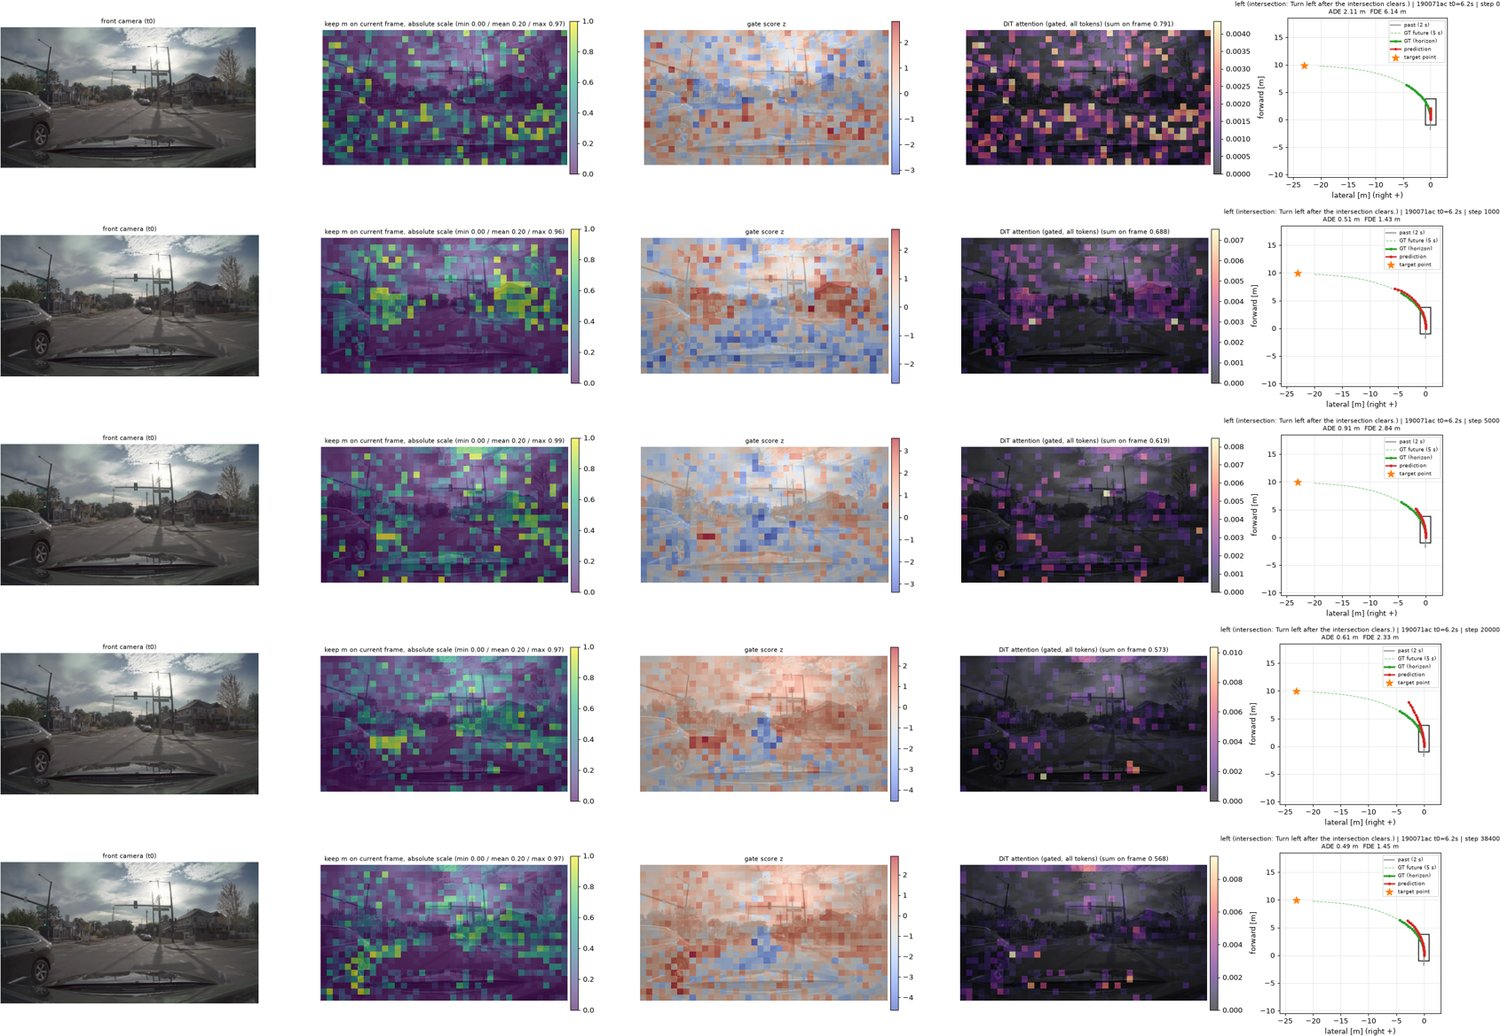
\includegraphics[width=\linewidth]{figures/evo_left.jpg}
\caption{Mask on one validation sample across training: steps 0, 1,000, 5,000, 20,000, 38,400, top to bottom. Panels as logged, left to right: current front frame; keep value $m$; standardized gate score $z$; DiT attention on the frame; bird's-eye view with past, ground truth, prediction and target point (lateral axis positive to the right).}
\label{fig:evo_left}
\end{figure}

\begin{figure}[h!]
\centering
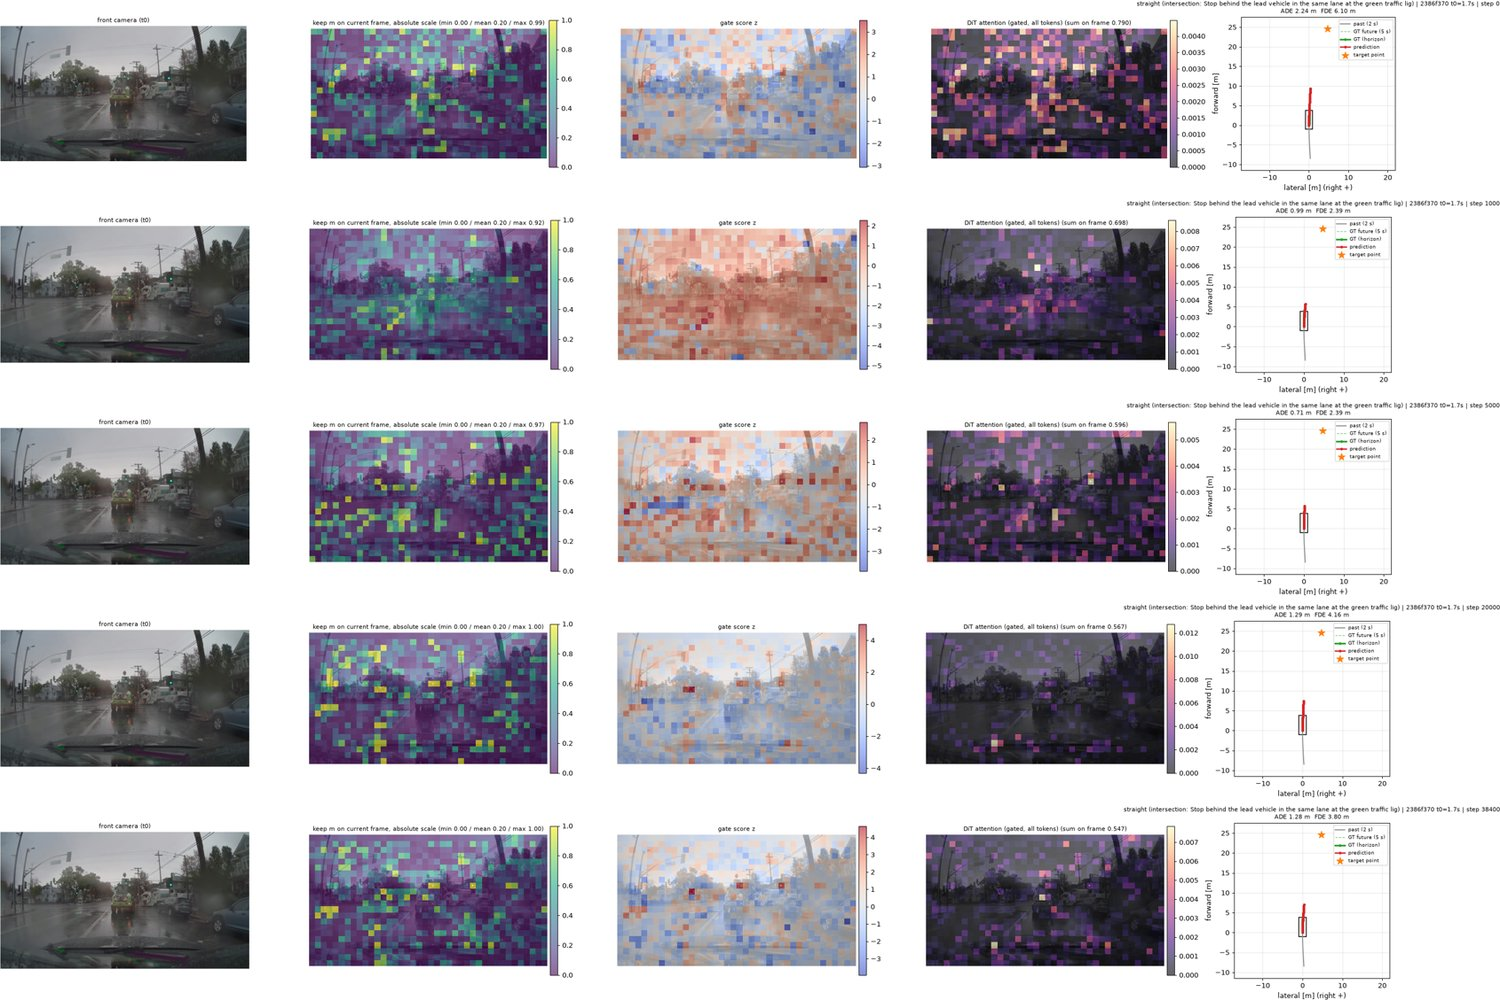
\includegraphics[width=\linewidth]{figures/evo_straight.jpg}
\caption{As Fig.~\ref{fig:evo_left}, for a straight sample behind a lead vehicle.}
\label{fig:evo_straight}
\end{figure}

\begin{figure}[h!]
\centering
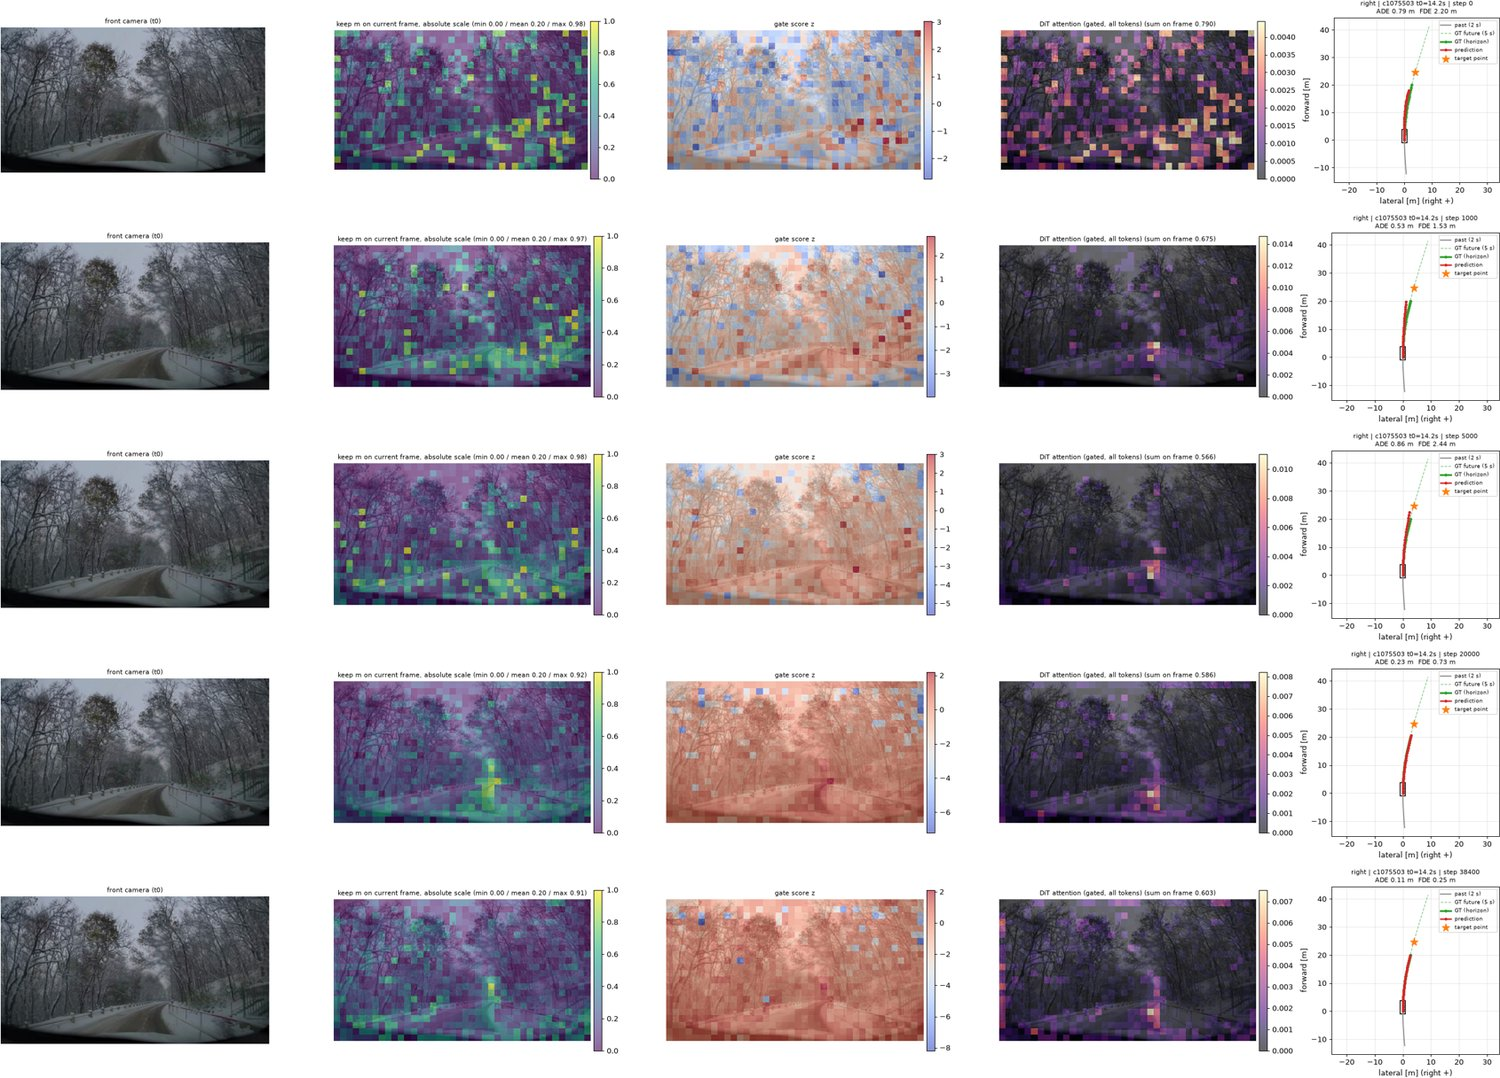
\includegraphics[width=\linewidth]{figures/evo_right.jpg}
\caption{As Fig.~\ref{fig:evo_left}, for a right-turn sample.}
\label{fig:evo_right}
\end{figure}

\clearpage
\begin{figure}[h!]
\centering
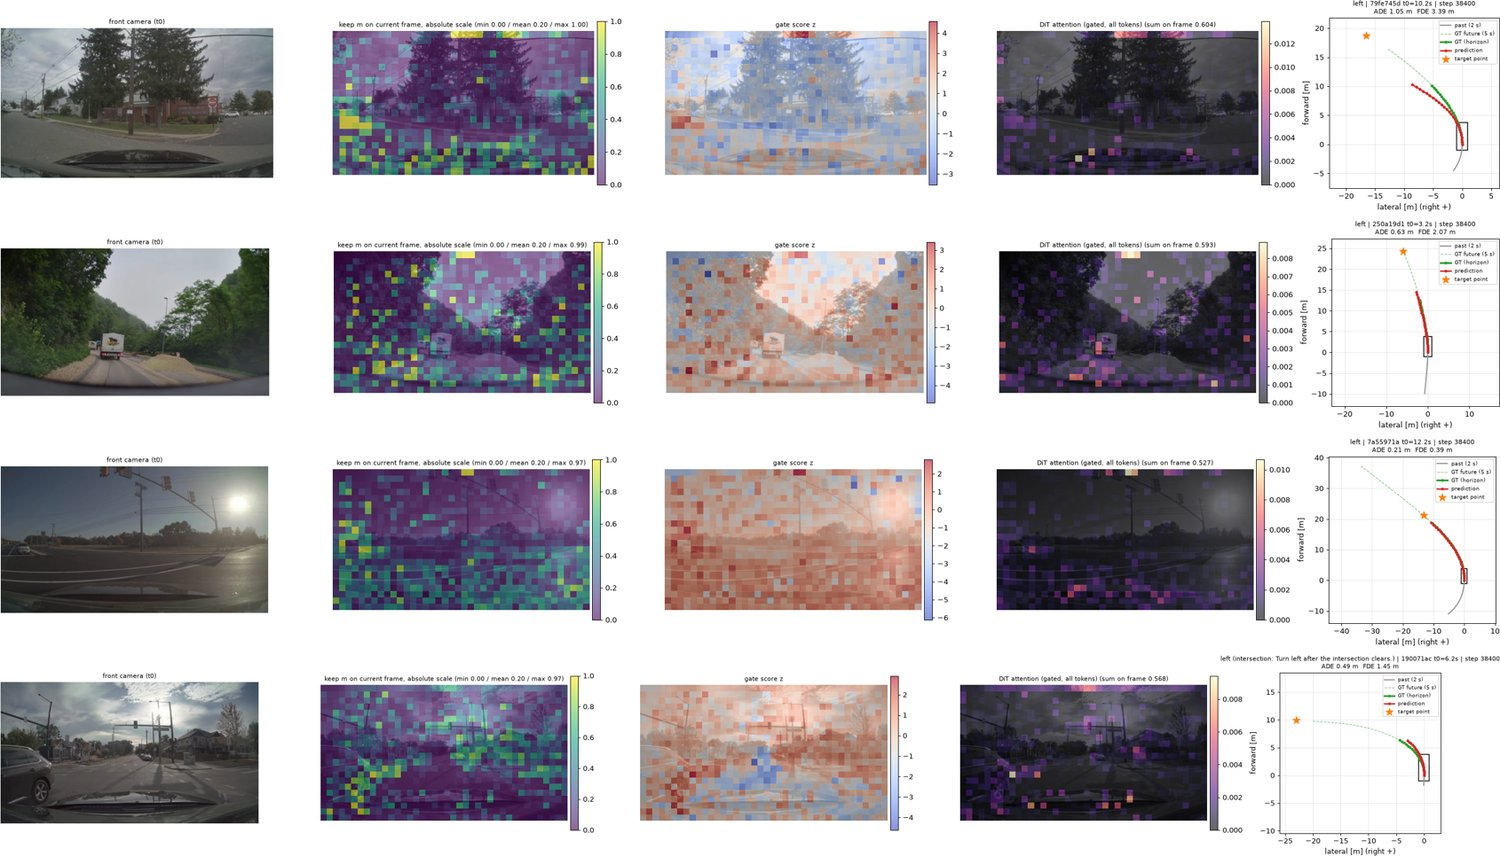
\includegraphics[width=\linewidth]{figures/final_left.jpg}
\caption{Mask-run left-turn samples at step 38{,}400. Panels as logged, left to right: current front frame; keep value $m$; standardized gate score $z$; DiT attention on the frame; bird's-eye view with past, ground truth, prediction and target point (lateral axis positive to the right).}
\label{fig:final_left}
\end{figure}

\begin{figure}[h!]
\centering
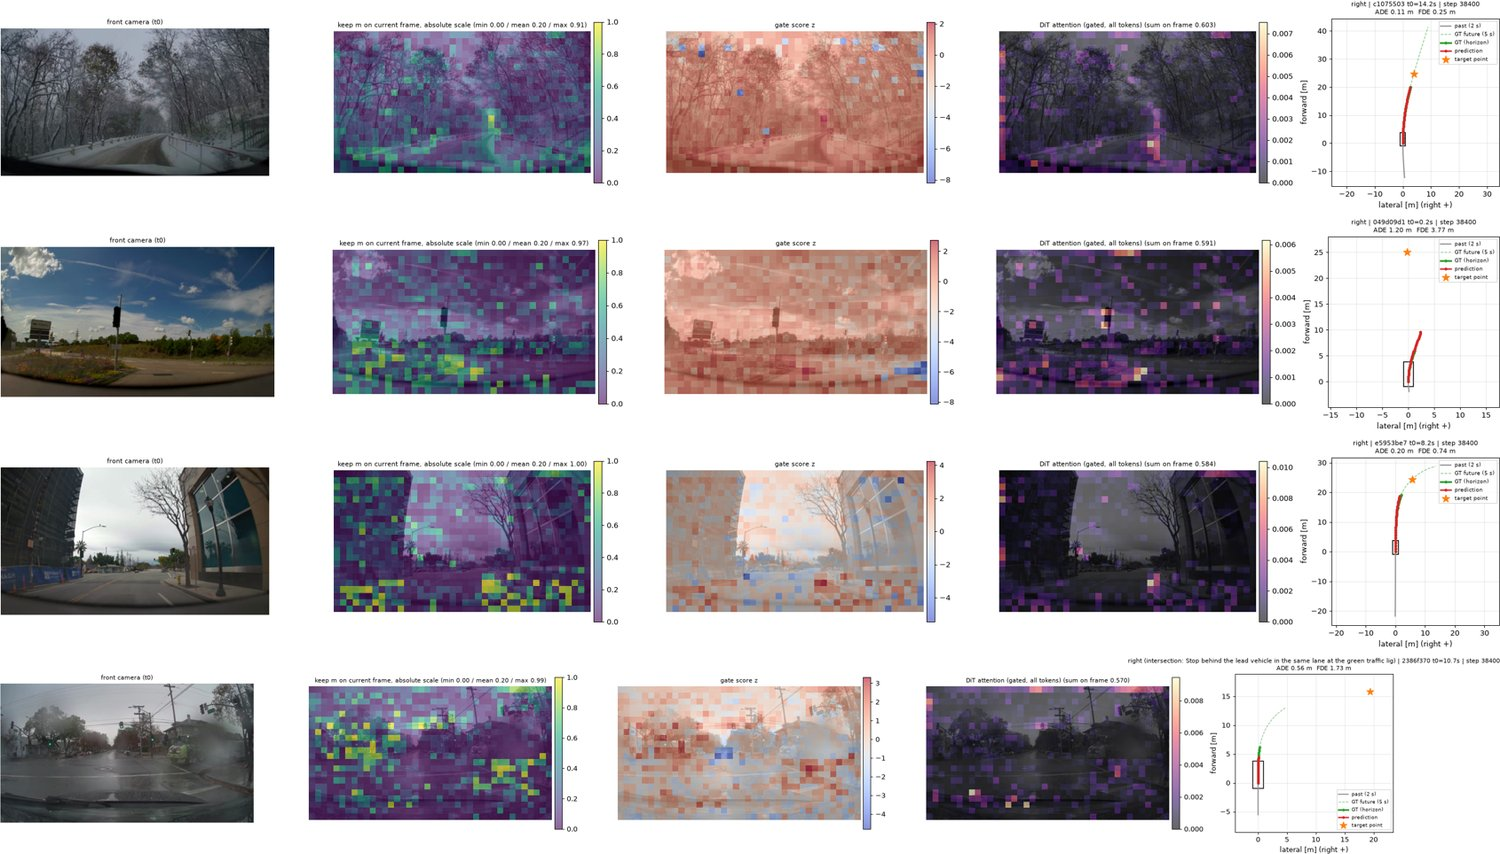
\includegraphics[width=\linewidth]{figures/final_right.jpg}
\caption{Mask-run right-turn samples at step 38{,}400, panels as in Fig.~\ref{fig:final_left}.}
\label{fig:final_right}
\end{figure}

\begin{figure}[h!]
\centering
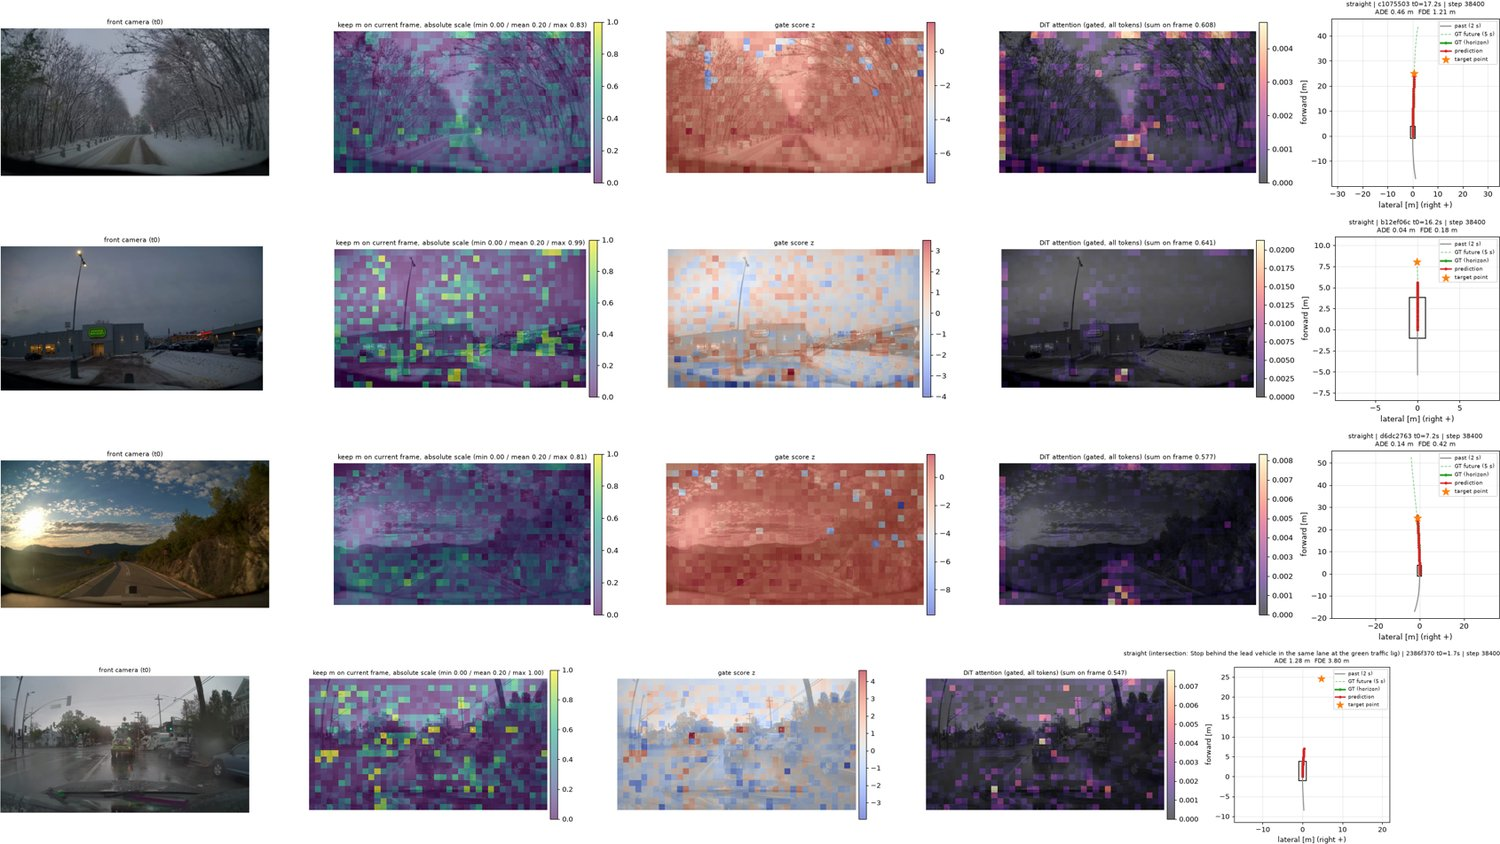
\includegraphics[width=\linewidth]{figures/final_straight.jpg}
\caption{Mask-run straight samples at step 38{,}400, panels as in Fig.~\ref{fig:final_left}.}
\label{fig:final_straight}
\end{figure}

\clearpage
\begin{figure}[h!]
\centering
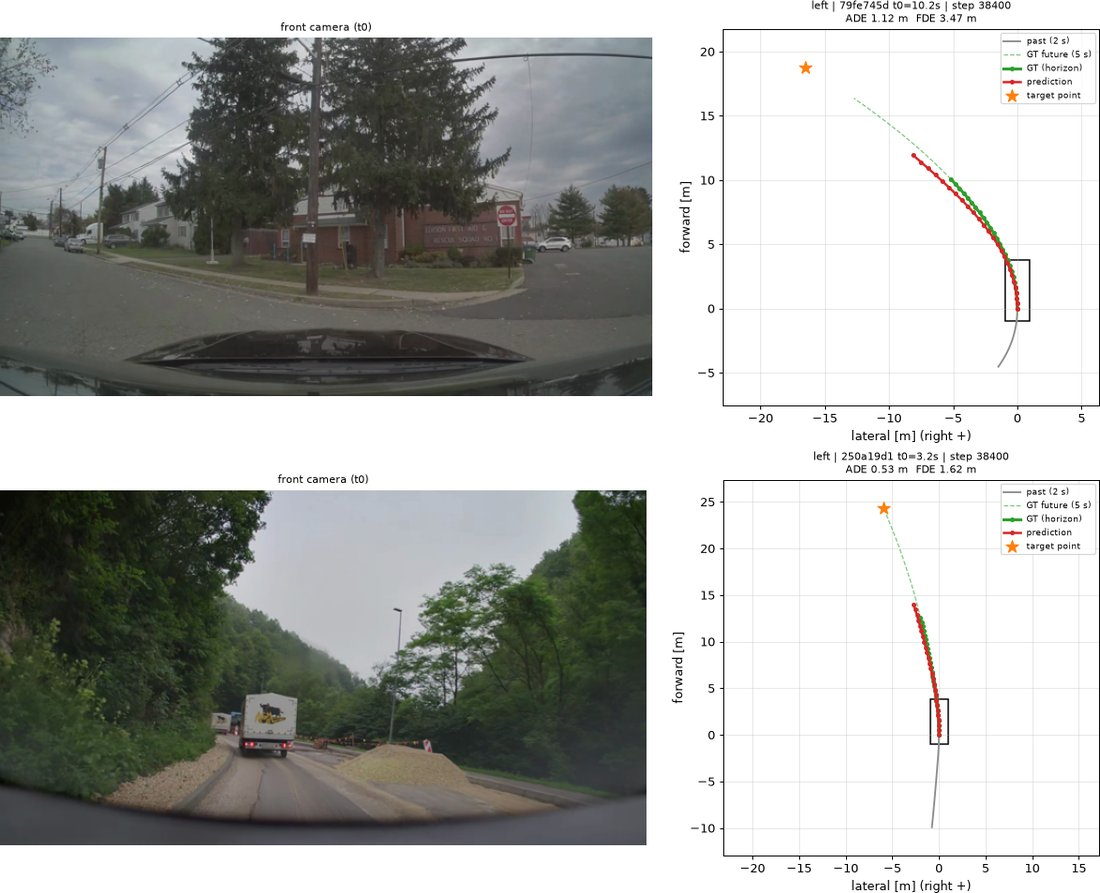
\includegraphics[width=0.8\linewidth]{figures/final_base_left.jpg}
\caption{Baseline on the first two left-turn samples of Fig.~\ref{fig:final_left}, step 38{,}400 (front frame and bird's-eye view; the baseline has no mask).}
\label{fig:base_left}
\end{figure}

\begin{figure}[h!]
\centering
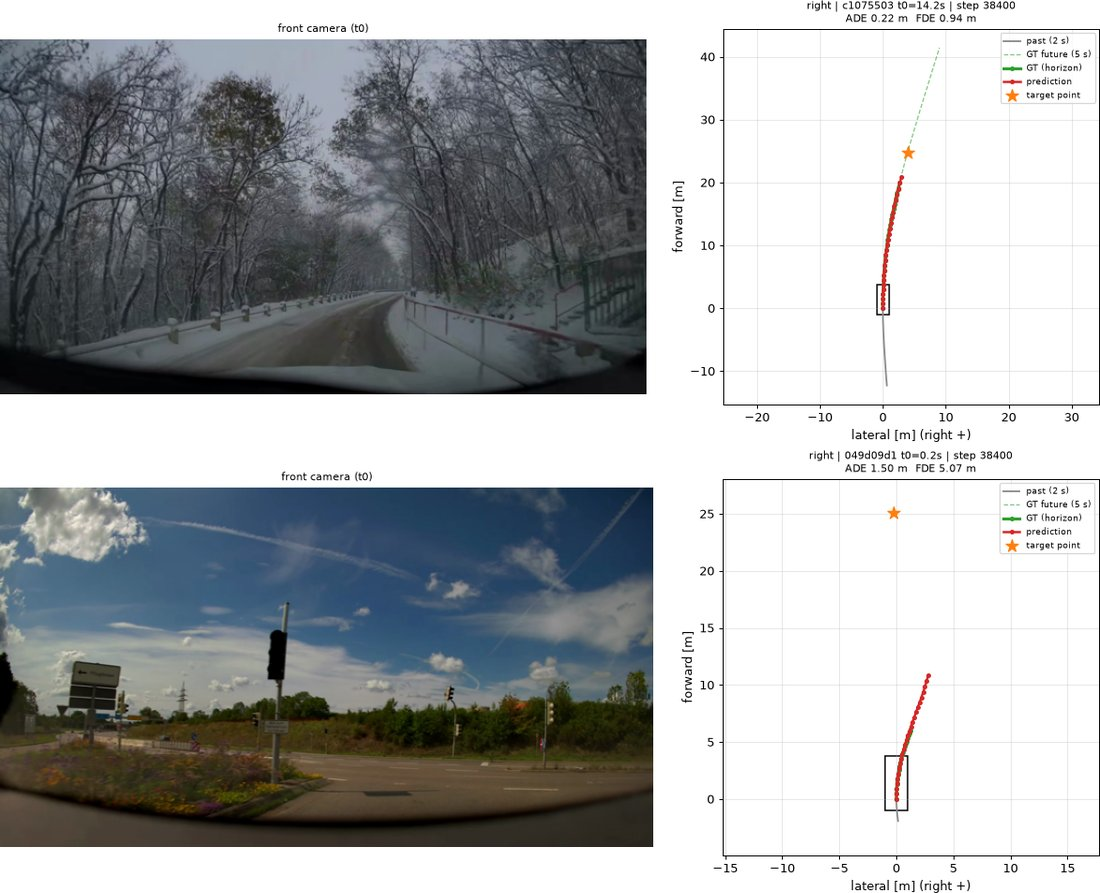
\includegraphics[width=0.8\linewidth]{figures/final_base_right.jpg}
\caption{Baseline on the first two right-turn samples of Fig.~\ref{fig:final_right}.}
\label{fig:base_right}
\end{figure}

\begin{figure}[h!]
\centering
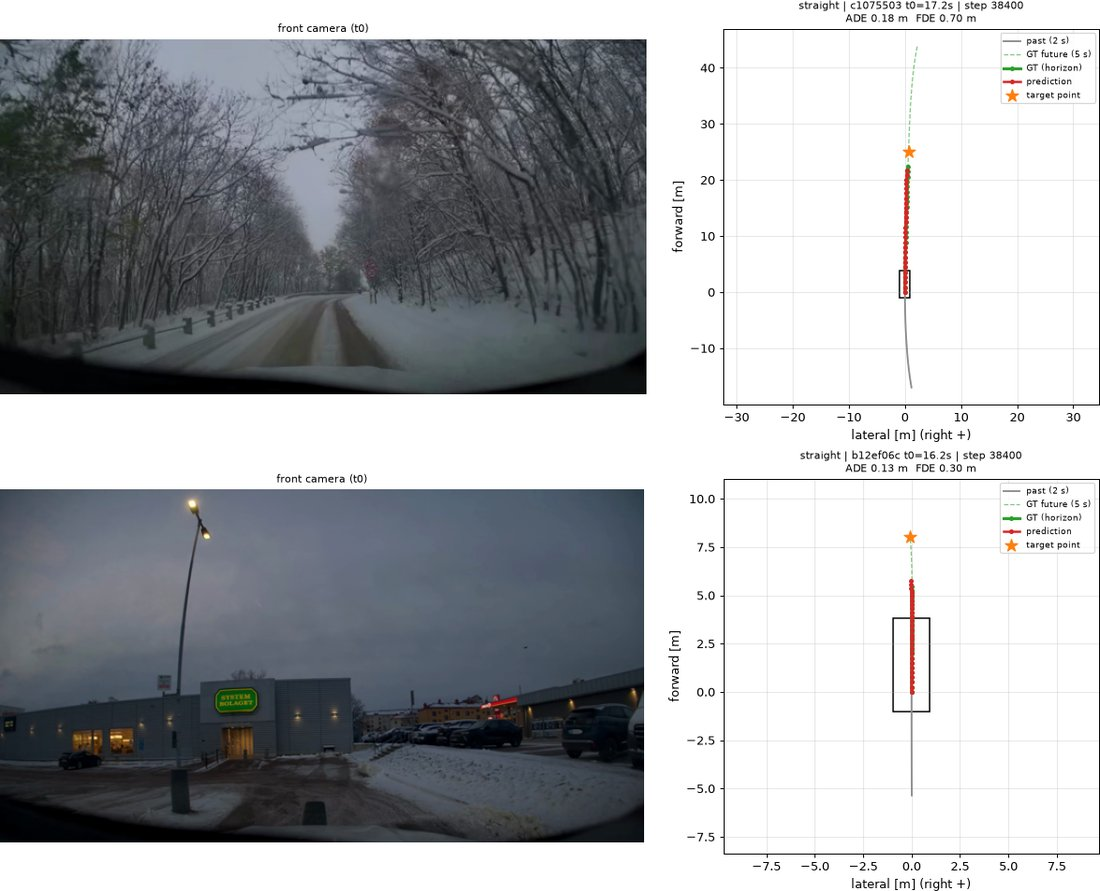
\includegraphics[width=0.8\linewidth]{figures/final_base_straight.jpg}
\caption{Baseline on the first two straight samples of Fig.~\ref{fig:final_straight}.}
\label{fig:base_straight}
\end{figure}

\clearpage
\begin{figure}[h!]
\centering
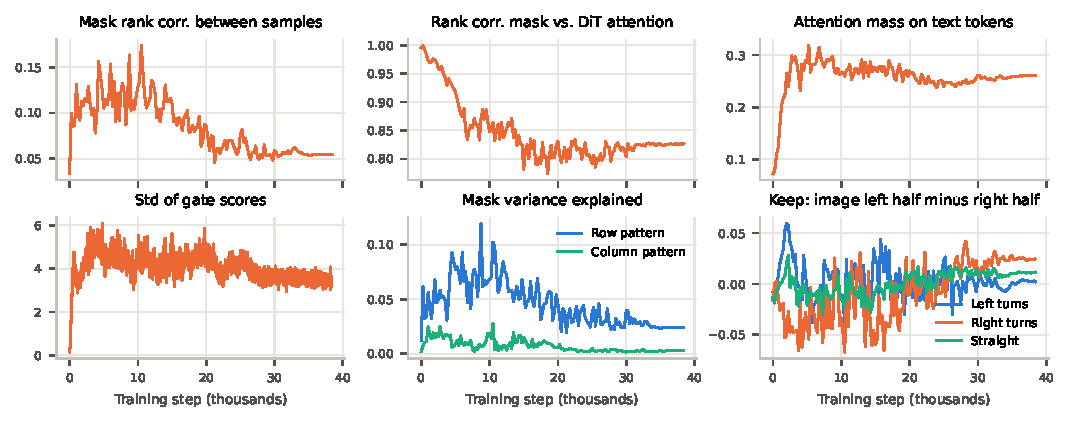
\includegraphics[width=\linewidth]{figures/curve_mask.pdf}
\caption{Mask diagnostics over training. The mask's rank correlation with DiT attention falls from near 1 to about 0.83, attention on text tokens rises early, and row and column patterns explain little of the mask's variance.}
\label{fig:curve_mask}
\end{figure}

\begin{figure}[h!]
\centering
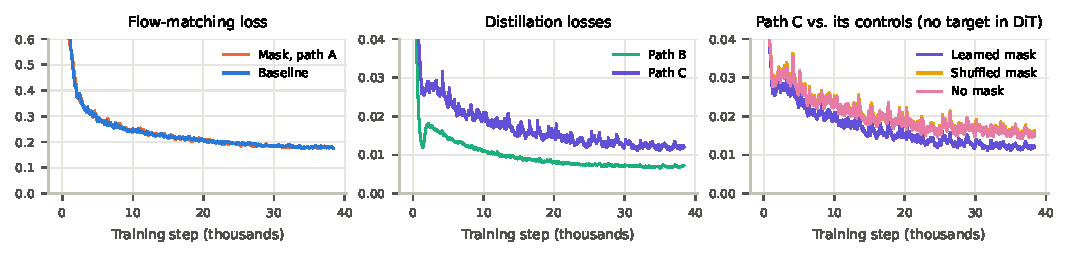
\includegraphics[width=\linewidth]{figures/curve_losses.pdf}
\caption{Training losses, smoothed (EMA 0.05). Baseline and path A match. Learned-mask path C stays below its shuffled and no-mask controls.}
\label{fig:curve_losses}
\end{figure}

\section{Open-loop results in full}
\label{app:open}
Both runs use the final checkpoint. The best evaluation over training is lower than the final one, on this fixed set of 240 samples: baseline ADE 0.302 at step 32,250 (final 0.337), mask 0.324 at step 34,750 (final 0.341). We did not select on this set. Each evaluation draws one flow-matching sample per input, so these values carry sampling noise; no confidence intervals were computed.

\begin{figure}[h!]
\centering
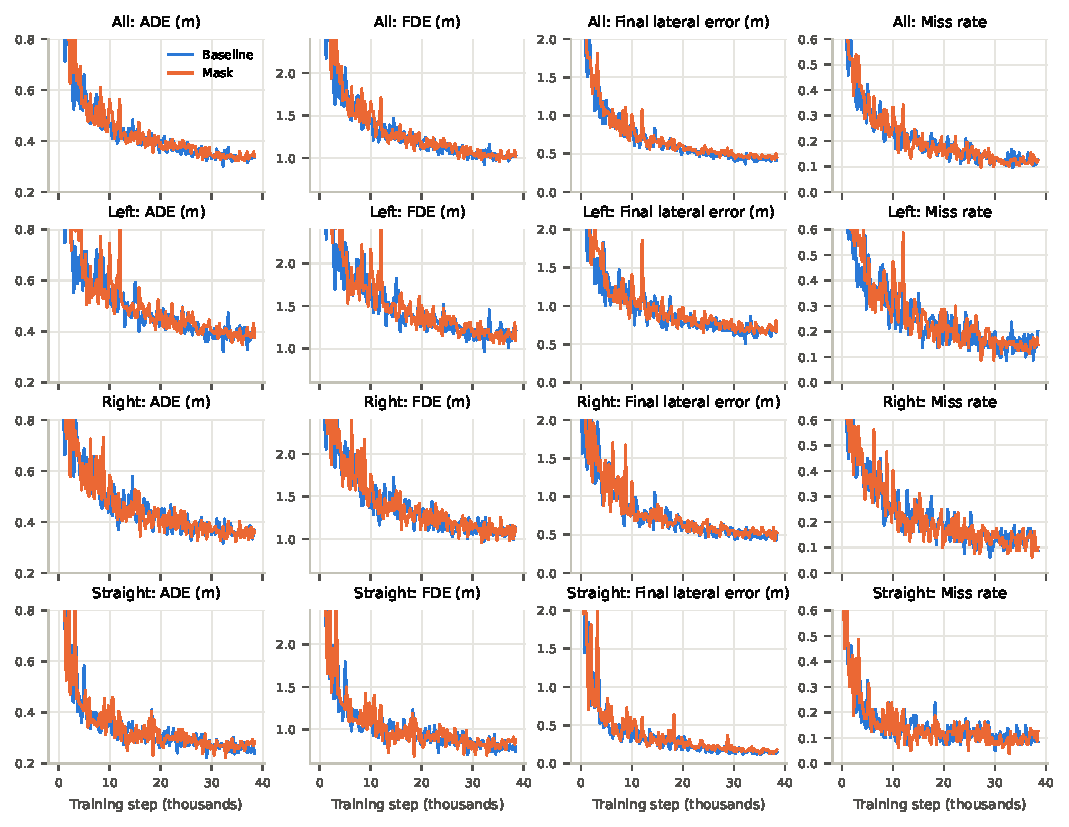
\includegraphics[width=\linewidth]{figures/curve_openloop.pdf}
\caption{Validation metrics over training, every 250 steps. Vertical axes are clipped, so the first evaluations are off scale.}
\label{fig:curve_openloop}
\end{figure}

\begin{figure}[h!]
\centering
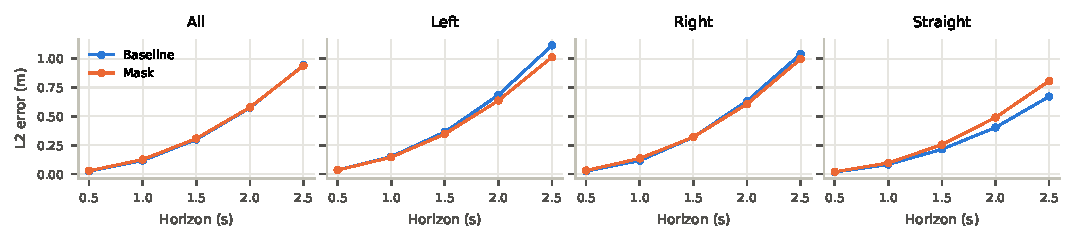
\includegraphics[width=\linewidth]{figures/horizon_error.pdf}
\caption{L2 error along the 2.5\,s horizon at step 38{,}400.}
\label{fig:horizon}
\end{figure}

\begin{figure}[h!]
\centering
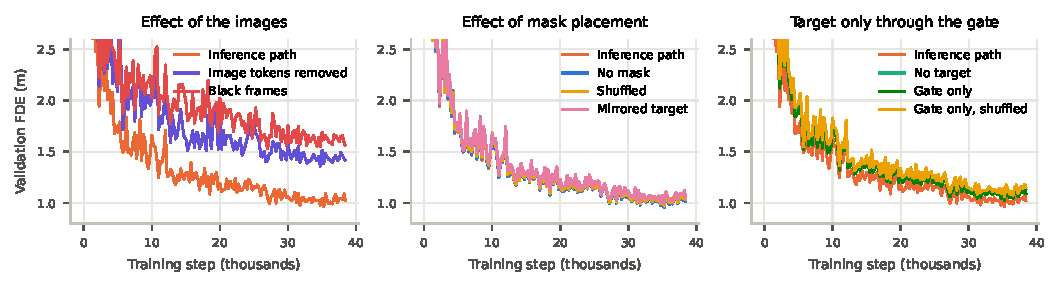
\includegraphics[width=\linewidth]{figures/curve_controls.pdf}
\caption{Mask-run evaluation controls over training (validation FDE). Definitions in Appendix~\ref{app:mask}.}
\label{fig:curve_controls}
\end{figure}

\begin{table}[h!]
\centering\scriptsize
\caption{Open-loop metrics at step 38{,}400 on the 240 fixed validation samples (m; miss rate as a fraction). L2 at the stated horizon in s; Lat./Lon.: absolute final error.}
\label{tab:app_open}
\begin{tabular}{llcccccccccc}
\toprule
 & Run & ADE & FDE & L2@0.5 & L2@1.0 & L2@1.5 & L2@2.0 & L2@2.5 & Lat. & Lon. & Miss \\
\midrule
All & Baseline & 0.337 & 1.029 & 0.025 & 0.117 & 0.300 & 0.574 & 0.943 & 0.478 & 0.802 & 0.125 \\
 & Mask & 0.341 & 1.023 & 0.028 & 0.126 & 0.308 & 0.578 & 0.939 & 0.457 & 0.796 & 0.125 \\
\midrule
Left & Baseline & 0.405 & 1.213 & 0.034 & 0.151 & 0.365 & 0.686 & 1.115 & 0.768 & 0.790 & 0.200 \\
 & Mask & 0.376 & 1.100 & 0.034 & 0.146 & 0.347 & 0.637 & 1.014 & 0.667 & 0.712 & 0.150 \\
\midrule
Right & Baseline & 0.367 & 1.136 & 0.025 & 0.117 & 0.320 & 0.633 & 1.041 & 0.516 & 0.931 & 0.087 \\
 & Mask & 0.360 & 1.089 & 0.031 & 0.136 & 0.321 & 0.606 & 0.997 & 0.526 & 0.867 & 0.100 \\
\midrule
Straight & Baseline & 0.239 & 0.737 & 0.017 & 0.083 & 0.215 & 0.404 & 0.672 & 0.149 & 0.686 & 0.087 \\
 & Mask & 0.287 & 0.879 & 0.020 & 0.097 & 0.255 & 0.490 & 0.806 & 0.179 & 0.810 & 0.125 \\
\bottomrule
\end{tabular}
\end{table}

\begin{table}[h!]
\centering\tiny
\caption{Evaluation controls of the mask run at step 38{,}400, with the noise of the main prediction. Each cell group is ADE, FDE, miss rate.}
\label{tab:app_ctrl}
\begin{tabular}{lcccccccccccc}
\toprule
 & \multicolumn{3}{c}{All} & \multicolumn{3}{c}{Left} & \multicolumn{3}{c}{Right} & \multicolumn{3}{c}{Straight} \\
\midrule
Inference path & 0.341 & 1.023 & 0.125 & 0.376 & 1.100 & 0.150 & 0.360 & 1.089 & 0.100 & 0.287 & 0.879 & 0.125 \\
\midrule
No mask & 0.339 & 1.016 & 0.129 & 0.376 & 1.096 & 0.138 & 0.358 & 1.086 & 0.125 & 0.282 & 0.866 & 0.125 \\
Shuffled mask & 0.344 & 1.031 & 0.133 & 0.382 & 1.115 & 0.150 & 0.363 & 1.099 & 0.125 & 0.287 & 0.879 & 0.125 \\
Mirrored target in gate & 0.348 & 1.049 & 0.129 & 0.392 & 1.154 & 0.175 & 0.363 & 1.114 & 0.087 & 0.288 & 0.881 & 0.125 \\
No target in DiT, no mask & 0.367 & 1.135 & 0.167 & 0.395 & 1.217 & 0.188 & 0.403 & 1.261 & 0.163 & 0.303 & 0.926 & 0.150 \\
No target in DiT, mask & 0.359 & 1.094 & 0.142 & 0.383 & 1.150 & 0.163 & 0.391 & 1.210 & 0.125 & 0.302 & 0.921 & 0.138 \\
No target in DiT, shuffled mask & 0.374 & 1.155 & 0.163 & 0.406 & 1.249 & 0.175 & 0.411 & 1.285 & 0.175 & 0.305 & 0.932 & 0.138 \\
All image tokens removed & 0.456 & 1.418 & 0.242 & 0.469 & 1.449 & 0.263 & 0.507 & 1.601 & 0.275 & 0.393 & 1.204 & 0.188 \\
Black input frames & 0.486 & 1.564 & 0.304 & 0.518 & 1.598 & 0.362 & 0.561 & 1.882 & 0.375 & 0.379 & 1.211 & 0.175 \\
\midrule
Baseline, black frames & 0.441 & 1.408 & 0.246 & 0.528 & 1.602 & 0.300 & 0.476 & 1.568 & 0.287 & 0.318 & 1.052 & 0.150 \\
\bottomrule
\end{tabular}
\end{table}

\begin{table}[h!]
\centering\tiny
\caption{Turn response at step 38{,}400. Direction accuracy and ratios use left/right samples with $|y_\mathrm{GT}|>0.5$\,m.}
\label{tab:app_turn}
\begin{tabular}{lccccccccc}
\toprule
 & Baseline & Mask & No mask & Shuffled & Mirrored & No target & No img tokens & Black & Base.\ black \\
\midrule
Corr.\ of final lateral offset & 0.986 & 0.987 & 0.987 & 0.987 & 0.986 & 0.984 & 0.967 & 0.959 & 0.969 \\
Std of predicted final lateral (m) & 4.451 & 4.482 & 4.488 & 4.497 & 4.384 & 4.475 & 3.981 & 3.668 & 3.993 \\
Left: direction accuracy & 0.987 & 1.000 & 1.000 & 1.000 & 0.987 & 1.000 & 1.000 & 1.000 & 0.987 \\
Right: direction accuracy & 1.000 & 1.000 & 1.000 & 1.000 & 1.000 & 0.987 & 0.973 & 1.000 & 0.973 \\
Left: median pred./GT lateral & 0.993 & 1.002 & 1.000 & 0.993 & 0.961 & 0.984 & 0.919 & 0.897 & 0.931 \\
Right: median pred./GT lateral & 1.031 & 1.020 & 1.018 & 1.025 & 0.973 & 0.986 & 0.823 & 0.726 & 0.838 \\
\bottomrule
\end{tabular}
\end{table}

\begin{figure}[h!]
\centering
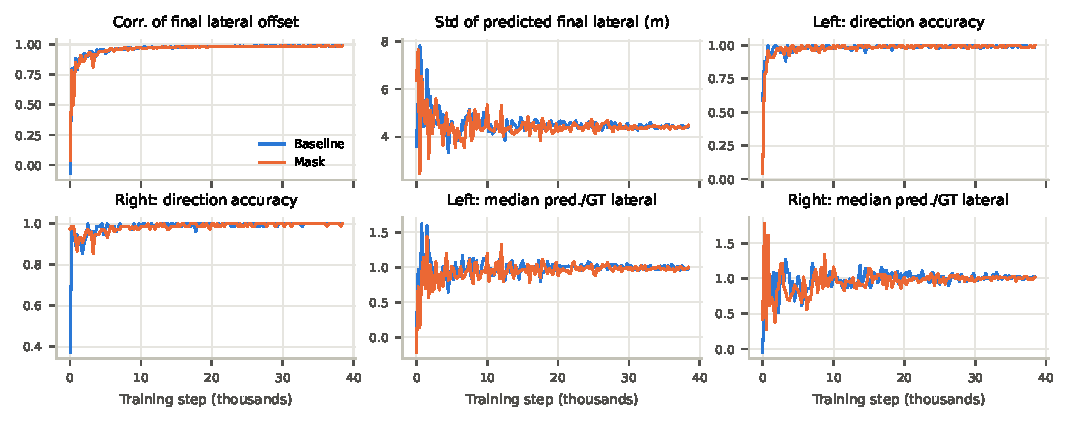
\includegraphics[width=\linewidth]{figures/curve_turn.pdf}
\caption{Turn response over training.}
\label{fig:curve_turn}
\end{figure}

\begin{figure}[h!]
\centering
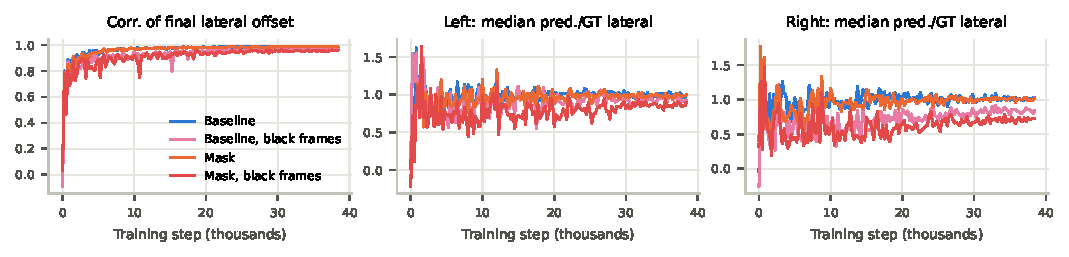
\includegraphics[width=\linewidth]{figures/curve_turn_noimage.pdf}
\caption{Turn response with the input frames replaced by black images.}
\label{fig:curve_turn_noimage}
\end{figure}

\begin{figure}[h!]
\centering
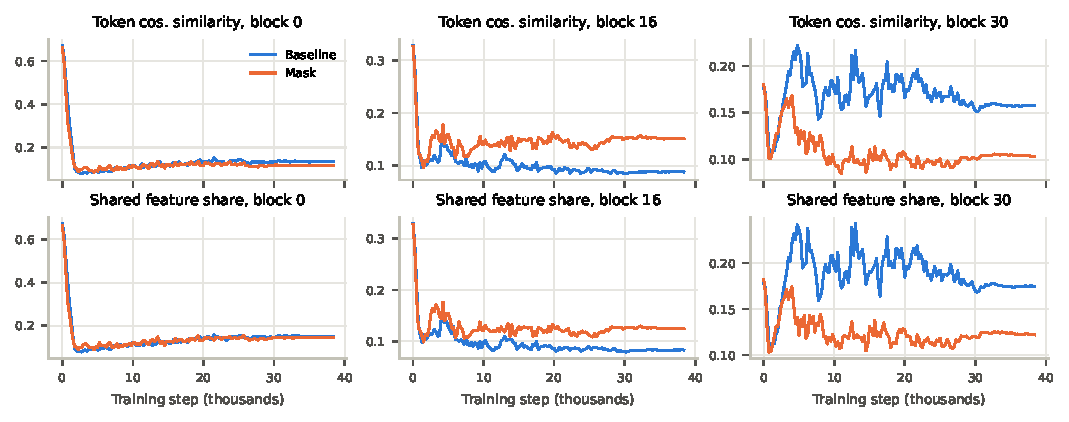
\includegraphics[width=\linewidth]{figures/curve_features.pdf}
\caption{How similar the VLM tokens entering the DiT are, at three DiT blocks. In the deep block the mask run's tokens are less alike than the baseline's.}
\label{fig:curve_features}
\end{figure}

\begin{figure}[h!]
\centering
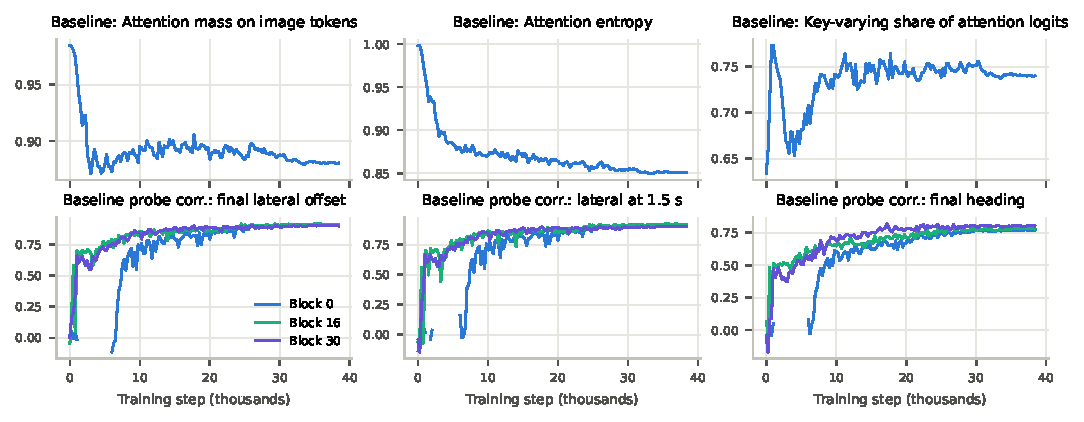
\includegraphics[width=\linewidth]{figures/curve_baseline_diag.pdf}
\caption{Baseline diagnostics: DiT attention statistics (top), and correlations of detached probes on projected VLM features at three blocks with future motion (bottom).}
\label{fig:curve_baseline_diag}
\end{figure}

\begin{figure}[h!]
\centering
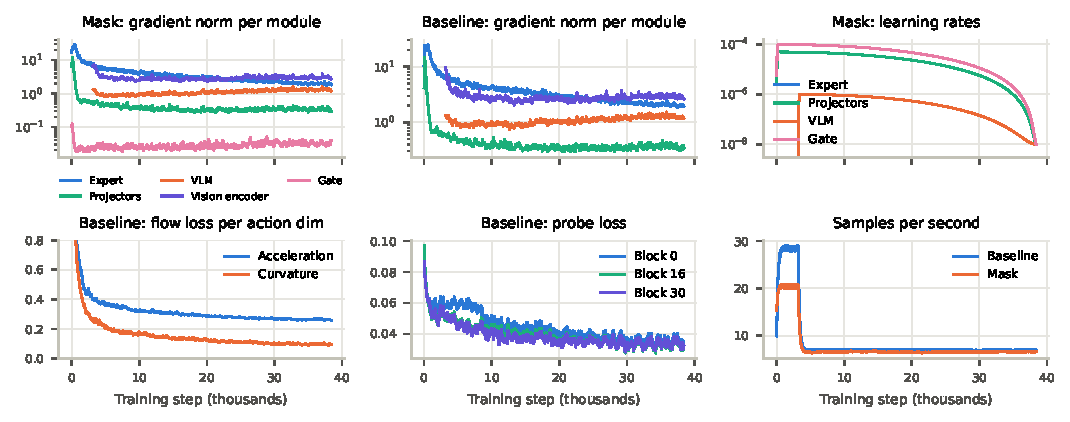
\includegraphics[width=\linewidth]{figures/curve_optim.pdf}
\caption{Optimization signals (smoothed). The first-epoch throughput is high because the VLM is frozen.}
\label{fig:curve_optim}
\end{figure}


\section{Driver pipeline}
\label{app:driver}
\textbf{Observation handling.} The driver answers AlpaSim's gRPC API. JPEGs of the mapped cameras are decoded on arrival; only the front wide camera feeds the policy and the detector. Calibration comes from the session's announced f-theta intrinsics, scaled to the decoded frame, with the rig file as a fallback. Egomotion is stamped on the newest observation bundle at every drive call, so the 0.5\,s replanning still reads a full 10\,Hz history.

\textbf{Route.} The challenge presets use MAP routes with a 40\,m start offset. When the route's first point is farther than the resampling step, a cubic Hermite curve leaving the rig origin along $+x$ and joining the route's first segment bridges the gap; the route is then extended beyond the farthest target distance and resampled at 0.1\,m. The target point is taken as in training, replacing the logged future with the route.

\textbf{Serving.} A plan is fixed in the local frame at creation. Each tick emits the plan's points at or after the current time on its own 10\,Hz grid. If a plan cannot be made (missing camera or ego pose, or a planning exception), the previous plan stays in use; with no usable plan, the driver serves a straight line at $\max(2\,\mathrm{m/s},v)$.

\textbf{AEB at a tick.} (1) If the newest front frame has not been processed and is due, run the detector and project the boxes. (2) Transform the rest of the cached plan to the rig frame and find the lead along it. (3) Update the track and compute the speed cap. (4) With a cap, let $w(\tau)$ be the distance the plan still means to cover in $\tau$ seconds, and $u(\tau)$ the distance allowed by the ramp (or $v\tau$ for the no-acceleration case). The served plan starts at the ego's projection onto the plan path, with arclength $s_\mathrm{ego}+\min(w,u)$ on a 0.1\,s grid and yaw interpolated along the path. (5) If the cap has just gone away, hold speed for this tick and drop the cached plan so that the next tick replans. Without step (5), the plan, now ahead of the braked ego, would make the controller accelerate toward what it braked for.

\section{AEB development}
\label{app:aeb}
\textbf{Why it was added.} Without AEB, the largest single loss is at-fault collisions, mostly front hits, and most of them involve a vehicle well below the ego's speed. Across 178 first-incident front hits in five runs (mask, TE4, hist\_ft, sig02), speed at impact has a median of 11.9\,m/s (quartiles 6.8 and 17.8). The last 3\,s are only moderately different from other 3\,s windows before any incident (6,077 windows): speed gain above 2\,m/s in 35\% vs.\ 25\%; mean acceleration above 0.3\,m/s$^2$ in 48\% vs.\ 37\%; peak above 1.5\,m/s$^2$ in 24\% vs.\ 21\%. A global acceleration limit would therefore mostly cost progress, so we chose a rule that looks at obstacles. The driver receives no other-actor state, and the recorded ground truth is off in the challenge presets, so obstacles must come from the cameras.

\textbf{Offline replay.} Each rollout log holds the front JPEGs, ego state and served plans. We ran the detector on them in the driver image and stored raw boxes, then evaluated the rule offline. A first version (no edge shrink, 1.6\,m corridor, trigger 2\,m/s$^2$) fired at least 1\,s before 38 of 41 front hits, but also fired in 29 of 46 sampled clean rollouts. Inspection traced this mainly to parked cars at the kerb: a box's bottom corners lie beside an obliquely seen vehicle and intrude into the corridor. Table~\ref{tab:app_sweep} shows the resulting trade-off. The replay is open loop and tuned on the evaluation scenes.

\begin{table}[h!]
\centering\tiny
\caption{Offline AEB threshold sweep on the replayed detections of the mask run's 150 rollouts (41 front hits, 62 rollouts without any incident). Brake counts only where the cap shortens the plan at 1\,s by over 0.3\,m. Chosen row in bold. Open loop: the ego does not react to the brake.}
\label{tab:app_sweep}
\begin{tabular}{cccccccc}
\toprule
Shrink & Half width & Trigger & Gap & Samples & Hits, $\ge1$\,s & Hits, $\ge0.5$\,s & Clean: rollouts / frames \\
\midrule
0.0 & 1.6 & 3.0 & 2.5 & 4 & 36 & 38 & 38 / 38 \\
0.3 & 1.3 & 4.0 & 1.5 & 6 & 24 & 28 & 28 / 15 \\
\textbf{0.3} & \textbf{1.3} & \textbf{3.0} & \textbf{2.5} & \textbf{6} & \textbf{29} & \textbf{32} & \textbf{32} / \textbf{19} \\
0.3 & 1.3 & 4.0 & 2.5 & 6 & 29 & 32 & 32 / 17 \\
0.15 & 1.3 & 3.0 & 2.5 & 6 & 32 & 37 & 37 / 22 \\
0.15 & 1.45 & 3.0 & 2.5 & 6 & 34 & 38 & 38 / 24 \\
0.3 & 1.6 & 3.0 & 2.5 & 6 & 31 & 36 & 36 / 22 \\
0.0 & 1.3 & 4.0 & 1.5 & 6 & 28 & 34 & 34 / 24 \\
0.3 & 1.3 & 2.0 & 2.5 & 6 & 31 & 32 & 32 / 23 \\
\bottomrule
\end{tabular}
\end{table}


\textbf{Chosen configuration.} For the chosen row, the no-acceleration rule (3\,s) adds 47 frames of intervention on clean rollouts. Rear-end collisions do not zero the score because only front and lateral collisions count as at fault, and progress saturates at 80\% of the recorded distance, so the score rewards this trade-off. This does not make the trade-off safe on a real road (Section~5).

\textbf{Detector choice.} RT-DETRv2 is available in the image's \texttt{transformers} with Apache-2.0 weights, and DETR-style output needs no NMS code. R18 and R50 were timed in the image on a busy RTX PRO 6000 Blackwell: about 38\,ms and 49\,ms median per frame, with 183 and 298\,MiB peak allocation. Resizing on the CPU and fp16 autocast did not change the R18 time (about 35\,ms), and a batch of 4 took the same time as a batch of 1 (about 30\,ms), so CPU-side kernel launches dominated under that host's load. CUDA-graph capture of the detector failed because the implementation writes to GPU tensors from the CPU in \texttt{forward}.

\section{Closed-loop results in full}
\label{app:closed}
\textbf{Protocol.} Scenes: a fixed 150-scene subset of the 441-scene \texttt{nurec\_curated\_val} suite. Preset \texttt{+e2e\_challenge=dev}, with a multi-GPU topology and driver recording on, on hosts shared with other jobs. First rollouts (baseline, mask, 10\,Hz AEB), TE4, hist\_ft and 8-sample ran on an RTX PRO 6000 Blackwell host (8 GPUs). Second rollouts, sig02 and 5\,Hz AEB ran on RTX 6000 Ada hosts (3 GPUs each). Every configuration therefore has its first and second rollout on different hardware, so the difference between a configuration's two rollouts mixes host and run-to-run variation. Scenes lost to renderer out-of-memory errors on shared GPUs were re-run, with fewer concurrent rollouts per renderer. Rollouts stop being scored at the first collision or offroad event. A rollout's score is 0 on an at-fault collision (front or lateral), offroad, or lateral corridor exit (over 4\,m from the recorded path), and otherwise $\min(\mathrm{progress}/0.8,1)$.

\begin{figure}[h!]
\centering
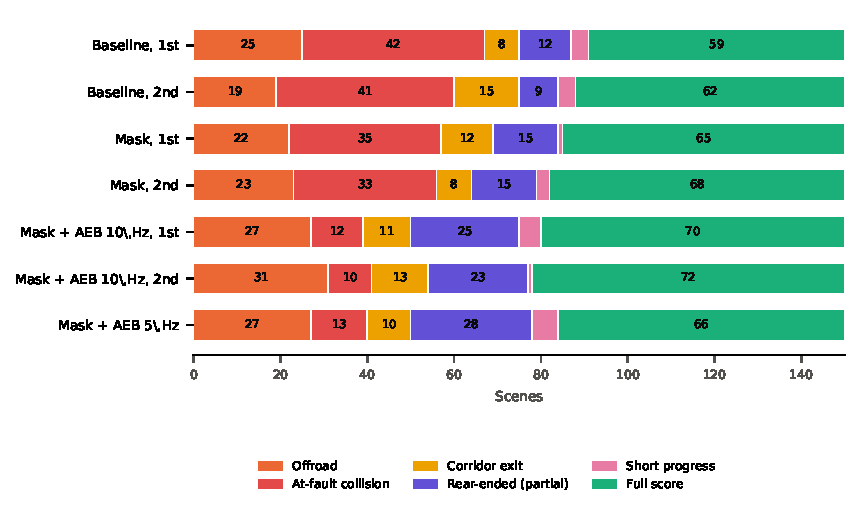
\includegraphics[width=0.85\linewidth]{figures/outcomes.pdf}
\caption{Outcome of each run on the same 150 scenes.}
\label{fig:outcomes}
\end{figure}

\begin{figure}[h!]
\centering
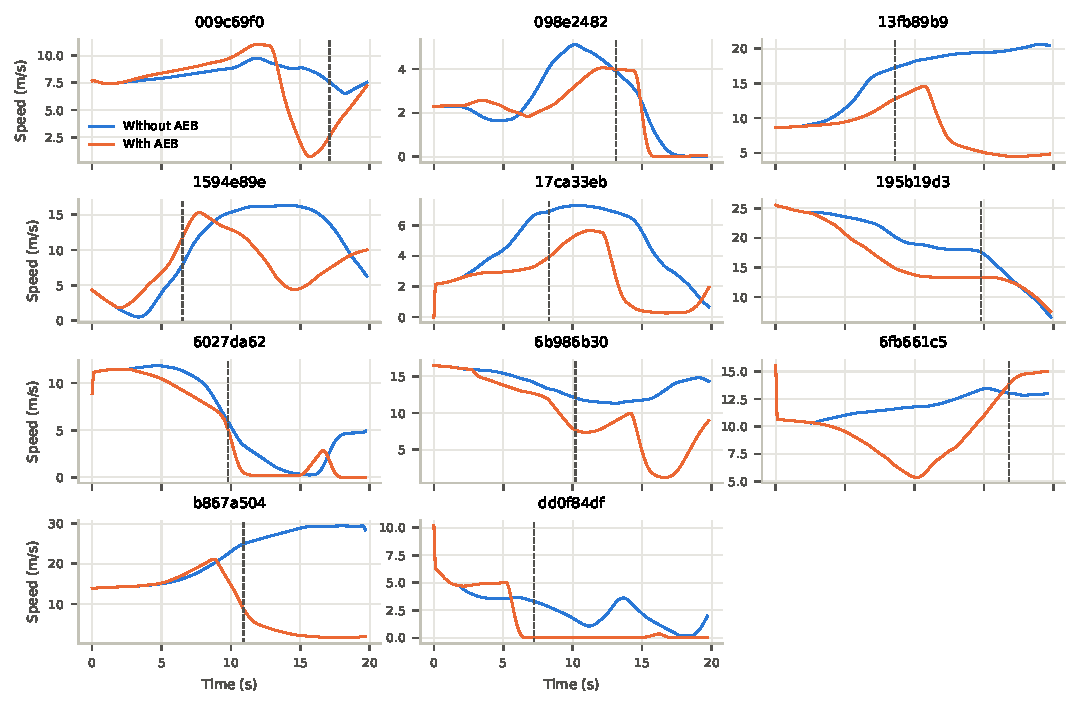
\includegraphics[width=\linewidth]{figures/aeb_speed.pdf}
\caption{Ego speed in the 11 scenes with an at-fault collision without AEB and a full score with it (first rollouts). Dashed: the collision without AEB.}
\label{fig:aeb_speed}
\end{figure}

\begin{figure}[h!]
\centering
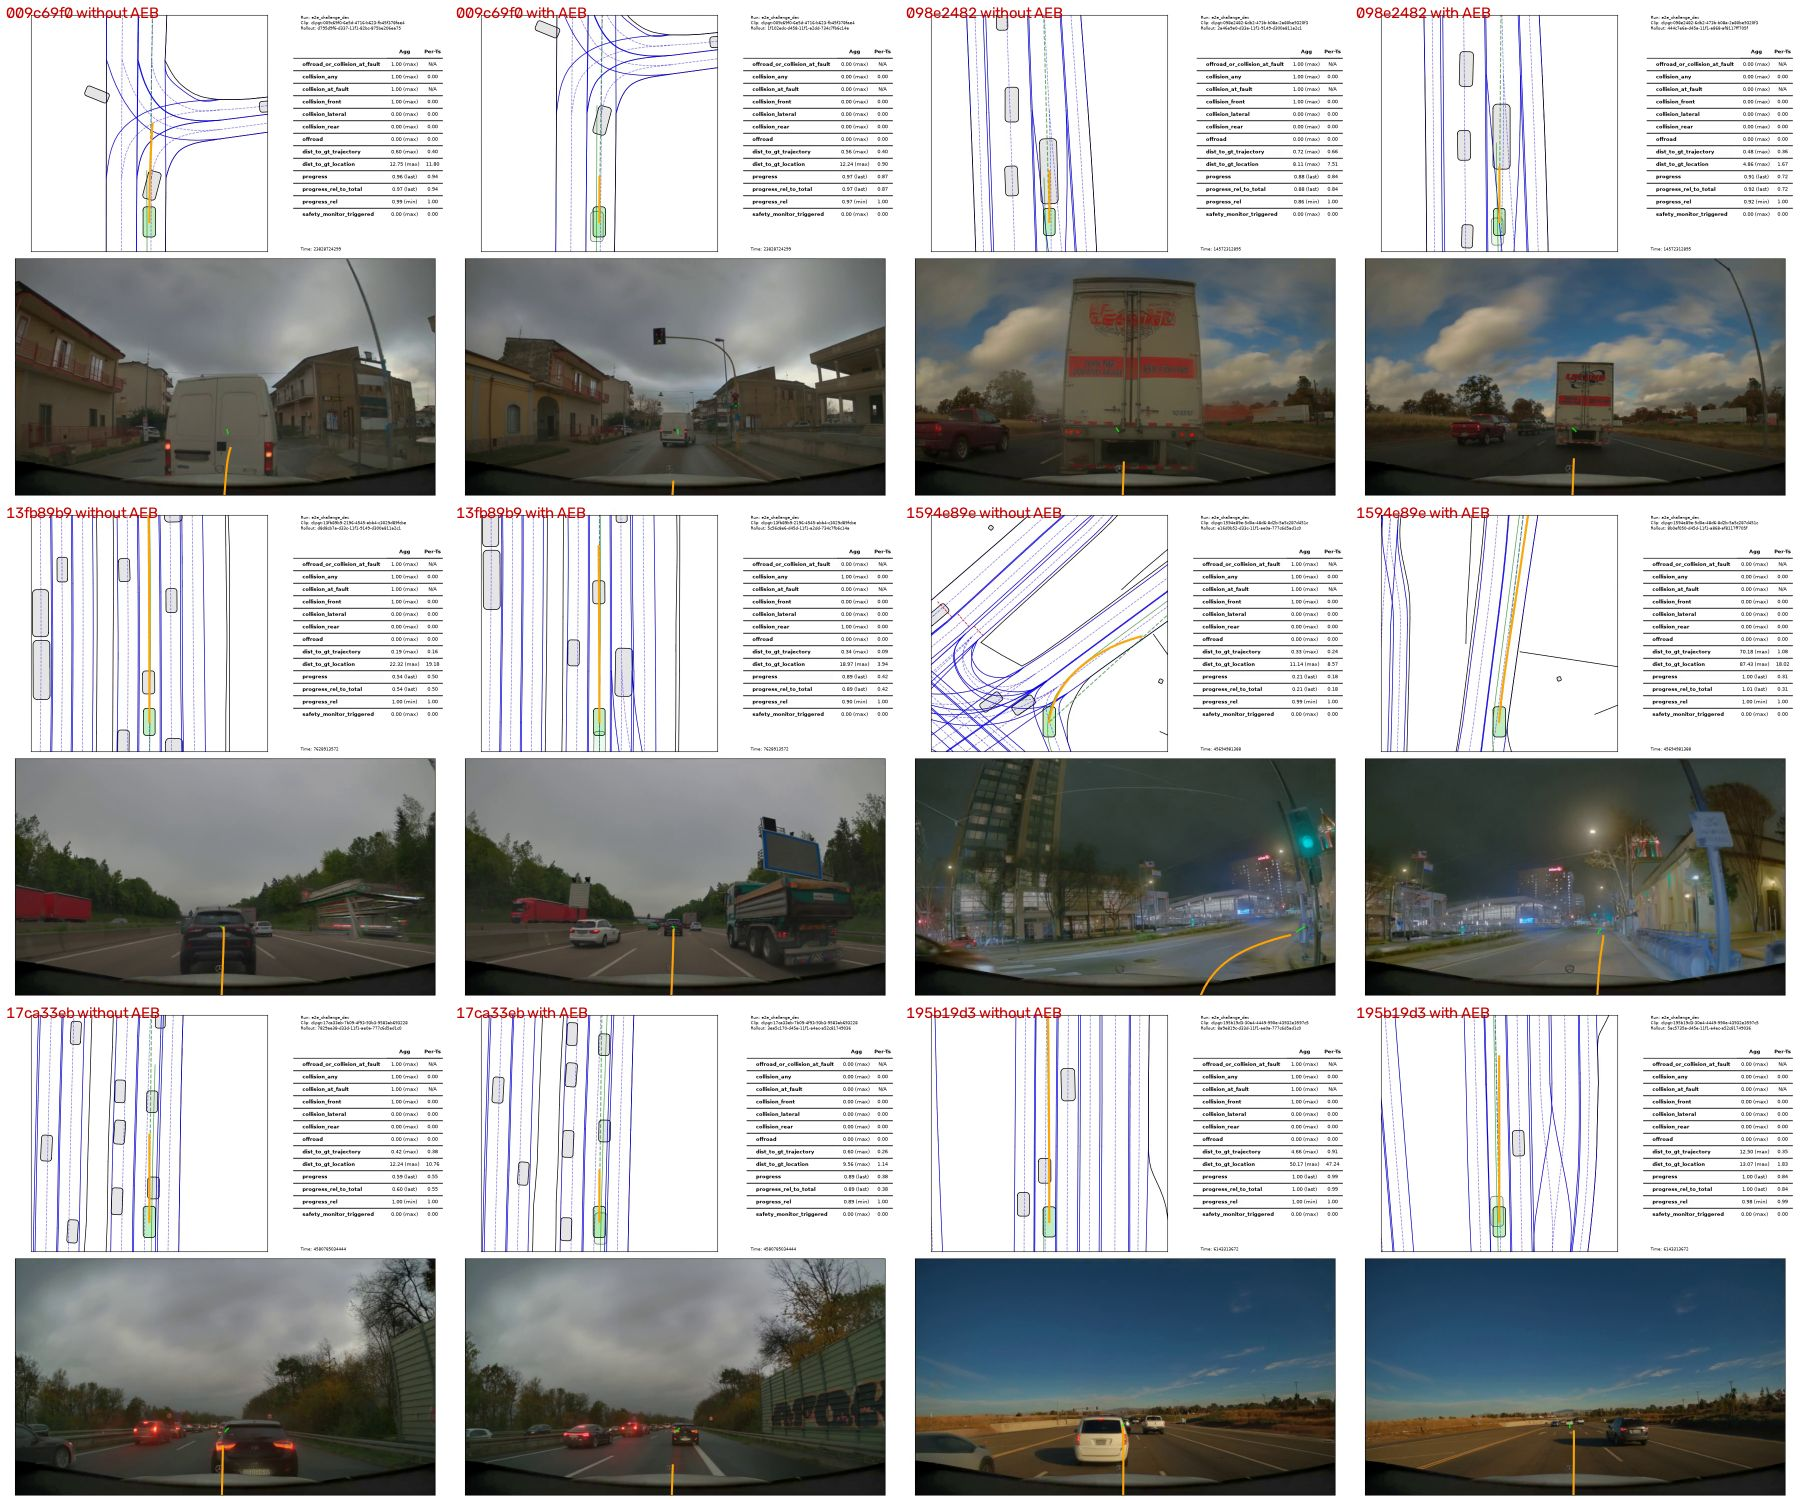
\includegraphics[width=\linewidth]{figures/aeb_pairs.jpg}
\caption{Same scene 0.3\,s before the collision without AEB, at the same time from rollout start with AEB (6 of the 11 scenes).}
\label{fig:aeb_pairs}
\end{figure}

\begin{figure}[h!]
\centering
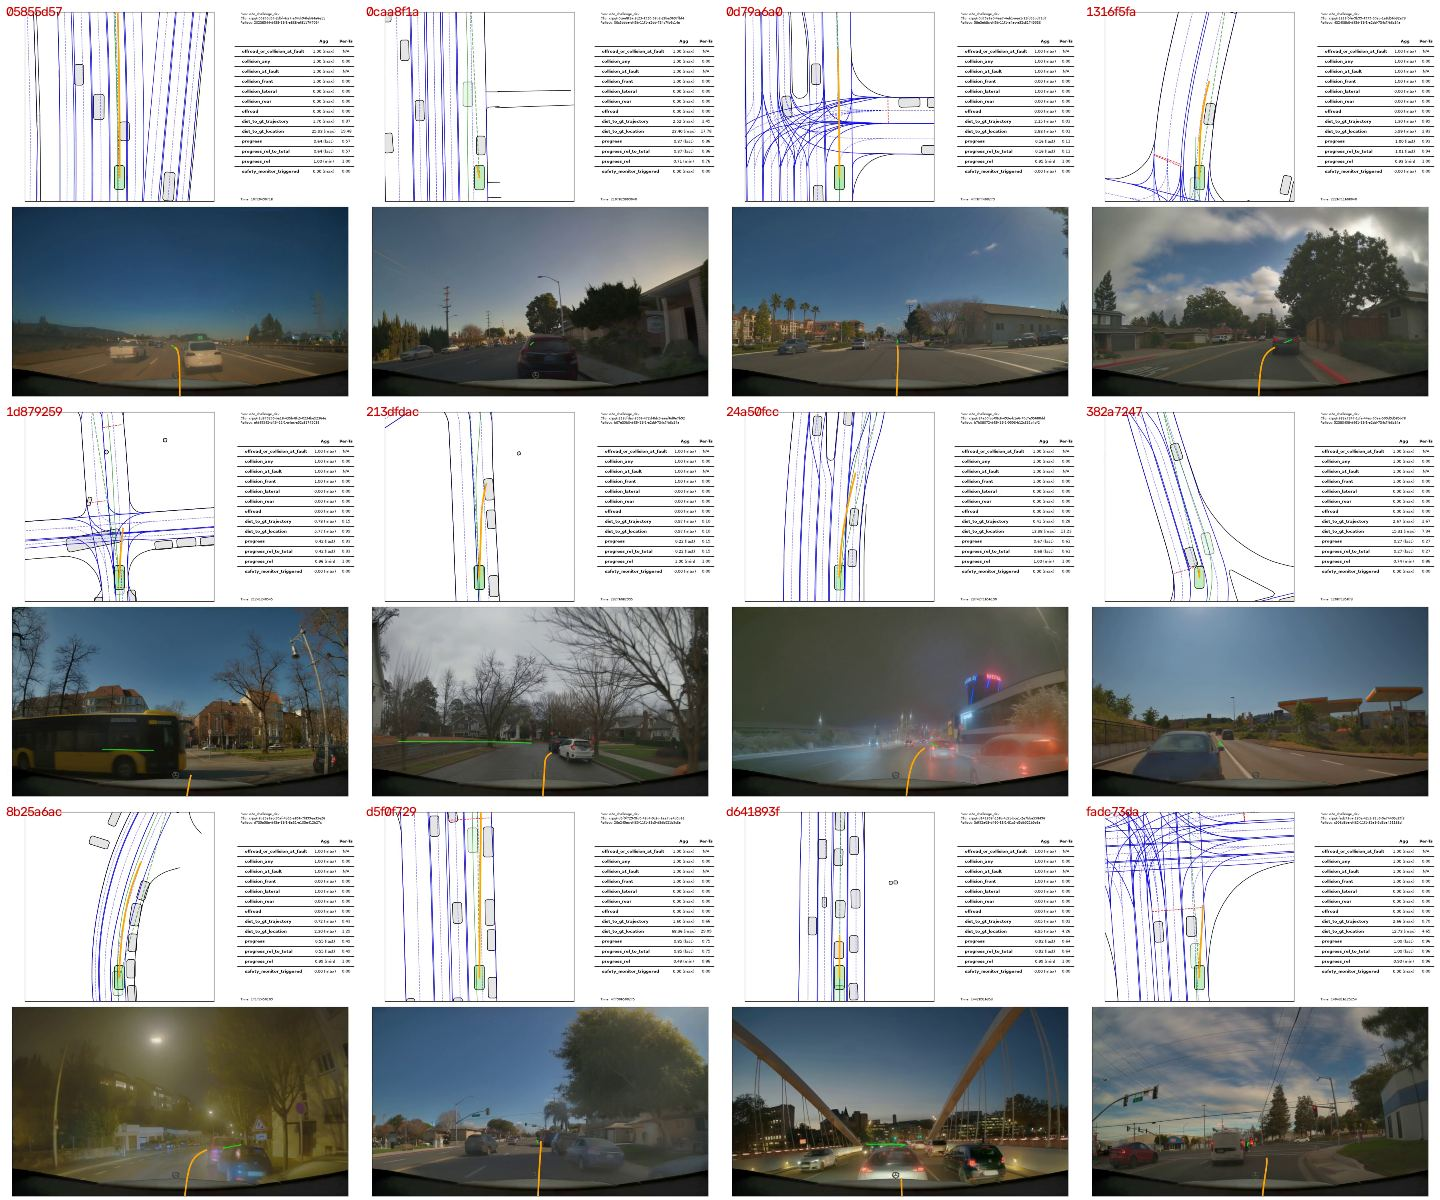
\includegraphics[width=\linewidth]{figures/sheet_collisions.jpg}
\caption{The 12 remaining at-fault collisions with AEB, 1\,s before the collision.}
\label{fig:sheet_collisions}
\end{figure}


\begin{table}[h!]
\centering\tiny
\caption{Score-loss decomposition on the same 150 scenes in every column: scenes / contribution to $1-\text{mean score}$.}
\label{tab:app_loss}
\begin{tabular}{lccccccc}
\toprule
 & Baseline, 1st & Baseline, 2nd & Mask, 1st & Mask, 2nd & AEB 10\,Hz, 1st & AEB 10\,Hz, 2nd & AEB 5\,Hz \\
\midrule
Offroad & 25 / 0.167 & 19 / 0.127 & 22 / 0.147 & 23 / 0.153 & 27 / 0.180 & 31 / 0.207 & 27 / 0.180 \\
At-fault collision & 42 / 0.280 & 41 / 0.273 & 35 / 0.233 & 33 / 0.220 & 12 / 0.080 & 10 / 0.067 & 13 / 0.087 \\
Corridor exit & 8 / 0.053 & 15 / 0.100 & 12 / 0.080 & 8 / 0.053 & 11 / 0.073 & 13 / 0.087 & 10 / 0.067 \\
Rear-ended (partial) & 12 / 0.022 & 9 / 0.015 & 15 / 0.038 & 15 / 0.037 & 25 / 0.054 & 23 / 0.046 & 28 / 0.067 \\
Short progress & 4 / 0.002 & 4 / 0.003 & 1 / 0.002 & 3 / 0.002 & 5 / 0.005 & 1 / 0.002 & 6 / 0.009 \\
Full score & 59 / 0.000 & 62 / 0.000 & 65 / 0.000 & 68 / 0.000 & 70 / 0.000 & 72 / 0.000 & 66 / 0.000 \\
\midrule
Mean score & 0.476 & 0.481 & 0.499 & 0.534 & 0.607 & 0.591 & 0.590 \\
Mean progress & 0.745 & 0.773 & 0.737 & 0.739 & 0.737 & 0.732 & 0.720 \\
Mean Drive (s) & 0.133 & 0.066 & 0.110 & 0.146 & 0.201 & 0.085 & 0.264 \\
Host & Blackwell & Ada & Blackwell & Ada & Blackwell & Ada & Ada \\
\bottomrule
\end{tabular}
\end{table}

\begin{table}[h!]
\centering\scriptsize
\caption{Paired per-scene comparisons on the same 150 scenes. CI: bootstrap with 10{,}000 resamples; $p$: two-sided sign test ignoring ties. Not corrected for multiple comparisons. (2): per-scene mean of two rollouts.}
\label{tab:app_pairs}
\begin{tabular}{lccccccc}
\toprule
Comparison & $n$ & Ref. & Run & Diff. & 95\% CI & W/L & $p$ \\
\midrule
Mask (2) vs.\ baseline (2) & 150 & 0.479 & 0.517 & +0.038 & [-0.018, +0.093] & 37/26 & 0.21 \\
Mask 1st vs.\ baseline 1st & 150 & 0.476 & 0.499 & +0.023 & [-0.049, +0.093] & 28/20 & 0.31 \\
Mask 2nd vs.\ baseline 2nd & 150 & 0.481 & 0.534 & +0.053 & [-0.022, +0.126] & 31/19 & 0.12 \\
Mask 2nd vs.\ mask 1st & 150 & 0.499 & 0.534 & +0.035 & [-0.017, +0.089] & 22/16 & 0.42 \\
Baseline 2nd vs.\ baseline 1st & 150 & 0.476 & 0.481 & +0.005 & [-0.065, +0.076] & 25/20 & 0.55 \\
AEB 10\,Hz (2) vs.\ mask (2) & 150 & 0.517 & 0.599 & +0.082 & [+0.023, +0.143] & 41/28 & 0.15 \\
AEB 10\,Hz 1st vs.\ mask 1st & 150 & 0.499 & 0.607 & +0.108 & [+0.038, +0.176] & 37/14 & $<$0.01 \\
AEB 10\,Hz 2nd vs.\ mask 2nd & 150 & 0.534 & 0.591 & +0.057 & [-0.024, +0.137] & 34/26 & 0.37 \\
AEB 10\,Hz 2nd vs.\ 1st & 150 & 0.607 & 0.591 & -0.016 & [-0.087, +0.054] & 24/30 & 0.50 \\
AEB 5\,Hz vs.\ mask (2) & 150 & 0.517 & 0.590 & +0.073 & [+0.012, +0.134] & 43/22 & 0.01 \\
AEB 5\,Hz vs.\ mask 2nd & 150 & 0.534 & 0.590 & +0.056 & [-0.013, +0.125] & 36/21 & 0.06 \\
AEB 5\,Hz vs.\ AEB 10\,Hz (2) & 150 & 0.599 & 0.590 & -0.009 & [-0.065, +0.044] & 34/34 & 1.00 \\
\bottomrule
\end{tabular}
\end{table}

\begin{table}[h!]
\centering\scriptsize
\caption{How scenes change when the AEB is added (first rollouts, same host, 150 scenes): row is the outcome without AEB, column with AEB.}
\label{tab:app_flow}
\begin{tabular}{lcccccc}
\toprule
Without $\backslash$ with & Offroad & Coll. & Exit & Rear & Short & Full \\
\midrule
Offroad & 19 &  & 1 &  &  & 2 \\
At-fault collision & 2 & 9 & 2 & 11 & 2 & 9 \\
Corridor exit & 3 &  & 5 & 1 &  & 3 \\
Rear-ended (partial) & 1 &  & 1 & 11 & 2 &  \\
Short progress &  &  &  &  & 1 &  \\
Full score & 2 & 3 & 2 & 2 &  & 56 \\
\bottomrule
\end{tabular}
\end{table}


\textbf{Collision kinematics without AEB.} Table~\ref{tab:app_kin} compares models. 
\begin{table}[h!]
\centering\scriptsize
\caption{First-incident front collisions on the same 150 scenes: rate; share with speed gain above 2\,m/s in the last 3\,s; share whose last plan did not slow down (planned speed 2\,s ahead $\ge v-0.3$\,m/s); share with the nearest actor ahead below 1\,m/s (approximate); median speed at impact (m/s).}
\label{tab:app_kin}
\begin{tabular}{lcccccc}
\toprule
 & Hits & Rate & Accel. & No slowing & Stopped lead & $v_\mathrm{hit}$ \\
\midrule
Baseline (2) & 90/301 & 29.9\% & 42\% & 68\% & 39\% & 11.6 \\
Mask (2) & 77/300 & 25.7\% & 30\% & 64\% & 38\% & 10.9 \\
Mask + AEB 10\,Hz (2) & 28/300 & 9.3\% & 32\% & 50\% & 61\% & 9.1 \\
Mask + AEB 5\,Hz & 12/150 & 8.0\% & 17\% & 42\% & 67\% & 2.4 \\
hist\_ft & 46/147 & 31.3\% & 46\% & 67\% & 39\% & 13.2 \\
sig02 & 50/150 & 33.3\% & 32\% & 62\% & 36\% & 12.9 \\
Mask + TE4 & 41/150 & 27.3\% & 29\% & 66\% & 34\% & 10.5 \\
Baseline + TE4 & 34/148 & 23.0\% & 35\% & 62\% & 44\% & 9.9 \\
\bottomrule
\end{tabular}
\end{table}


\textbf{Remaining collisions with AEB (first rollout).} Table~\ref{tab:app_hits} lists all 12. \emph{Corridor}: the obstacle was outside the corridor until shortly before the hit or throughout; with no edge shrink and a 2\,m half width, the same replay sees most of them earlier, at the price of the false brakes described above. \emph{Side/behind}: the actor approached from outside the corridor (crossing bus; vehicle from behind-left). \emph{Close range}: the estimated gap stayed near 4.4\,m, so no closing speed was seen; hood occlusion of the wheels is our hypothesis, not verified. \emph{Late brake}: in \texttt{1316f5fa}, a distance jump restarted the track, so braking began about 0.5\,s before the hit; in \texttt{382a7247}, the ego slowed from 9.2 to 0.7\,m/s and still touched.

\begin{table}[h!]
\centering\tiny
\caption{The 12 at-fault collisions with AEB (10\,Hz). Time from rollout start; speeds 3\,s before and at the hit; minimum acceleration in the last 3\,s; nearest other actor at the hit (speed, longitudinal and lateral centre offset in the ego frame, relative heading; approximate, it may not be the actor hit); seconds before the hit that the rule's brake condition first holds in detector replay. Classes are our judgment.}
\label{tab:app_hits}
\begin{tabular}{llcccccccccc}
\toprule
Scene & Class & Type & $t$ & $v_{-3}$ & $v$ & $a_\mathrm{min}$ & $v_o$ & Lon. & Lat. & Head. & Brake \\
\midrule
\texttt{0caa8f1a} & Close range & front & 9.4 & 0.1 & 1.2 & -1.5 & 0.5 & 4.4 & -1.4 & -10 & 4.5 \\
\texttt{d641893f} & Close range & front & 15.1 & 0.9 & 4.2 & 0.8 & 12.0 & -1.1 & 3.1 & -179 & none \\
\texttt{05855d57} & Corridor & front & 11.5 & 30.3 & 32.0 & -0.7 & 26.8 & 4.3 & -0.0 & 2 & 0.3 \\
\texttt{213dfdac} & Corridor & front & 3.2 & 11.3 & 8.7 & -1.5 & 0.1 & 2.2 & -1.9 & 7 & none \\
\texttt{24a50fcc} & Corridor & front & 11.3 & 9.8 & 9.7 & -0.7 & 7.1 & 1.9 & -1.9 & 4 & none \\
\texttt{8b25a6ac} & Corridor & side & 10.6 & 9.9 & 9.9 & -0.1 & 0.0 & 2.7 & -2.1 & -1 & none \\
\texttt{d5f0f729} & Corridor & front & 18.2 & 24.3 & 21.7 & -1.5 & 0.1 & 4.2 & -1.6 & 1 & none \\
\texttt{fadc73da} & Corridor & front & 17.1 & 1.4 & 6.5 & -0.2 & 0.0 & 3.7 & 2.1 & 4 & none \\
\texttt{1316f5fa} & Late brake & front & 19.8 & 6.6 & 7.0 & -8.3 & 0.1 & 4.3 & -1.7 & -5 & 0.5 \\
\texttt{382a7247} & Late brake & front & 9.0 & 9.2 & 0.7 & -8.6 & 0.0 & 4.0 & 1.8 & -162 & 2.9 \\
\texttt{0d79a6a0} & Side/behind & side & 3.2 & 10.5 & 8.1 & -5.5 & 11.8 & 0.1 & 2.5 & -22 & 0.9 \\
\texttt{1d879259} & Side/behind & front & 6.0 & 2.1 & 4.6 & -2.9 & 6.0 & 4.6 & -0.8 & -71 & 0.3 \\
\bottomrule
\end{tabular}
\end{table}


\textbf{Lateral failures with AEB (first rollout).} Of the 27 offroad scenes, 19 were also offroad in the first no-AEB rollout, and 3 had hard braking (below $-2$\,m/s$^2$) in the last 3\,s, so the AEB is not their main cause. 18 of 27 changed heading by less than $15^\circ$ in the last 3\,s, consistent with slow drift, and video of 12 sampled scenes often shows the plan heading to the right shoulder. Of 31 lateral failures with a measurable side, 17 are on the right and 9 on the left of the route, with 5 within 0.3\,m.

\textbf{Route as a lateral reference.} Routes are generated from map lanes, so they are a candidate lateral reference. Sampling every 2\,m and placing the ego footprint along the route, 114 of 36,843 poses (0.3\%) count as offroad under the scorer's logic (5,728 do not fit inside one lane but touch no road edge). So the route is almost always on the road, but Tables~\ref{tab:app_route} and~\ref{tab:app_guard} show that distance to it separates failures from normal driving poorly, so we did not deploy a guard.

\begin{table}[h!]
\centering\scriptsize
\caption{Ego distance to the served route before lateral failures with AEB (m). Scenes without a covering route segment are omitted. For comparison, frames of the 70 full-score rollouts: median 0.29, 90th percentile 1.14, 99th percentile 2.99.}
\label{tab:app_route}
\begin{tabular}{llcccccc}
\toprule
Failure & Before & $n$ & Median & p25 & p75 & $>1$\,m & $>2$\,m \\
\midrule
Offroad & $-3$\,s & 18 & 0.40 & 0.18 & 2.56 & 5 & 5 \\
 & $-2$\,s & 23 & 0.49 & 0.31 & 1.36 & 6 & 4 \\
 & $-1$\,s & 23 & 0.70 & 0.33 & 1.91 & 11 & 5 \\
 & $-0$\,s & 23 & 0.67 & 0.40 & 1.99 & 8 & 6 \\
\midrule
Corridor exit & $-3$\,s & 5 & 0.81 & 0.70 & 0.87 & 1 & 1 \\
 & $-2$\,s & 7 & 0.79 & 0.34 & 2.77 & 3 & 3 \\
 & $-1$\,s & 8 & 0.82 & 0.26 & 2.36 & 4 & 3 \\
 & $-0$\,s & 8 & 2.80 & 0.61 & 3.43 & 5 & 5 \\
\bottomrule
\end{tabular}
\end{table}

\begin{table}[h!]
\centering\scriptsize
\caption{Offline check of a route-distance guard (not deployed): lateral failures flagged at least 1\,s before the failure, and full-score rollouts ever flagged.}
\label{tab:app_guard}
\begin{tabular}{ccccc}
\toprule
Threshold (m) & Ego: failures & Ego: clean & Plan at 2\,s: failures & Plan at 2\,s: clean \\
\midrule
0.5 & 27/38 & 50/70 & 29/38 & 49/70 \\
0.75 & 21/38 & 37/70 & 26/38 & 39/70 \\
1.0 & 19/38 & 30/70 & 23/38 & 33/70 \\
1.5 & 15/38 & 17/70 & 17/38 & 20/70 \\
2.0 & 13/38 & 15/70 & 15/38 & 16/70 \\
3.0 & 8/38 & 7/70 & 12/38 & 9/70 \\
\bottomrule
\end{tabular}
\end{table}

\begin{figure}[h!]
\centering
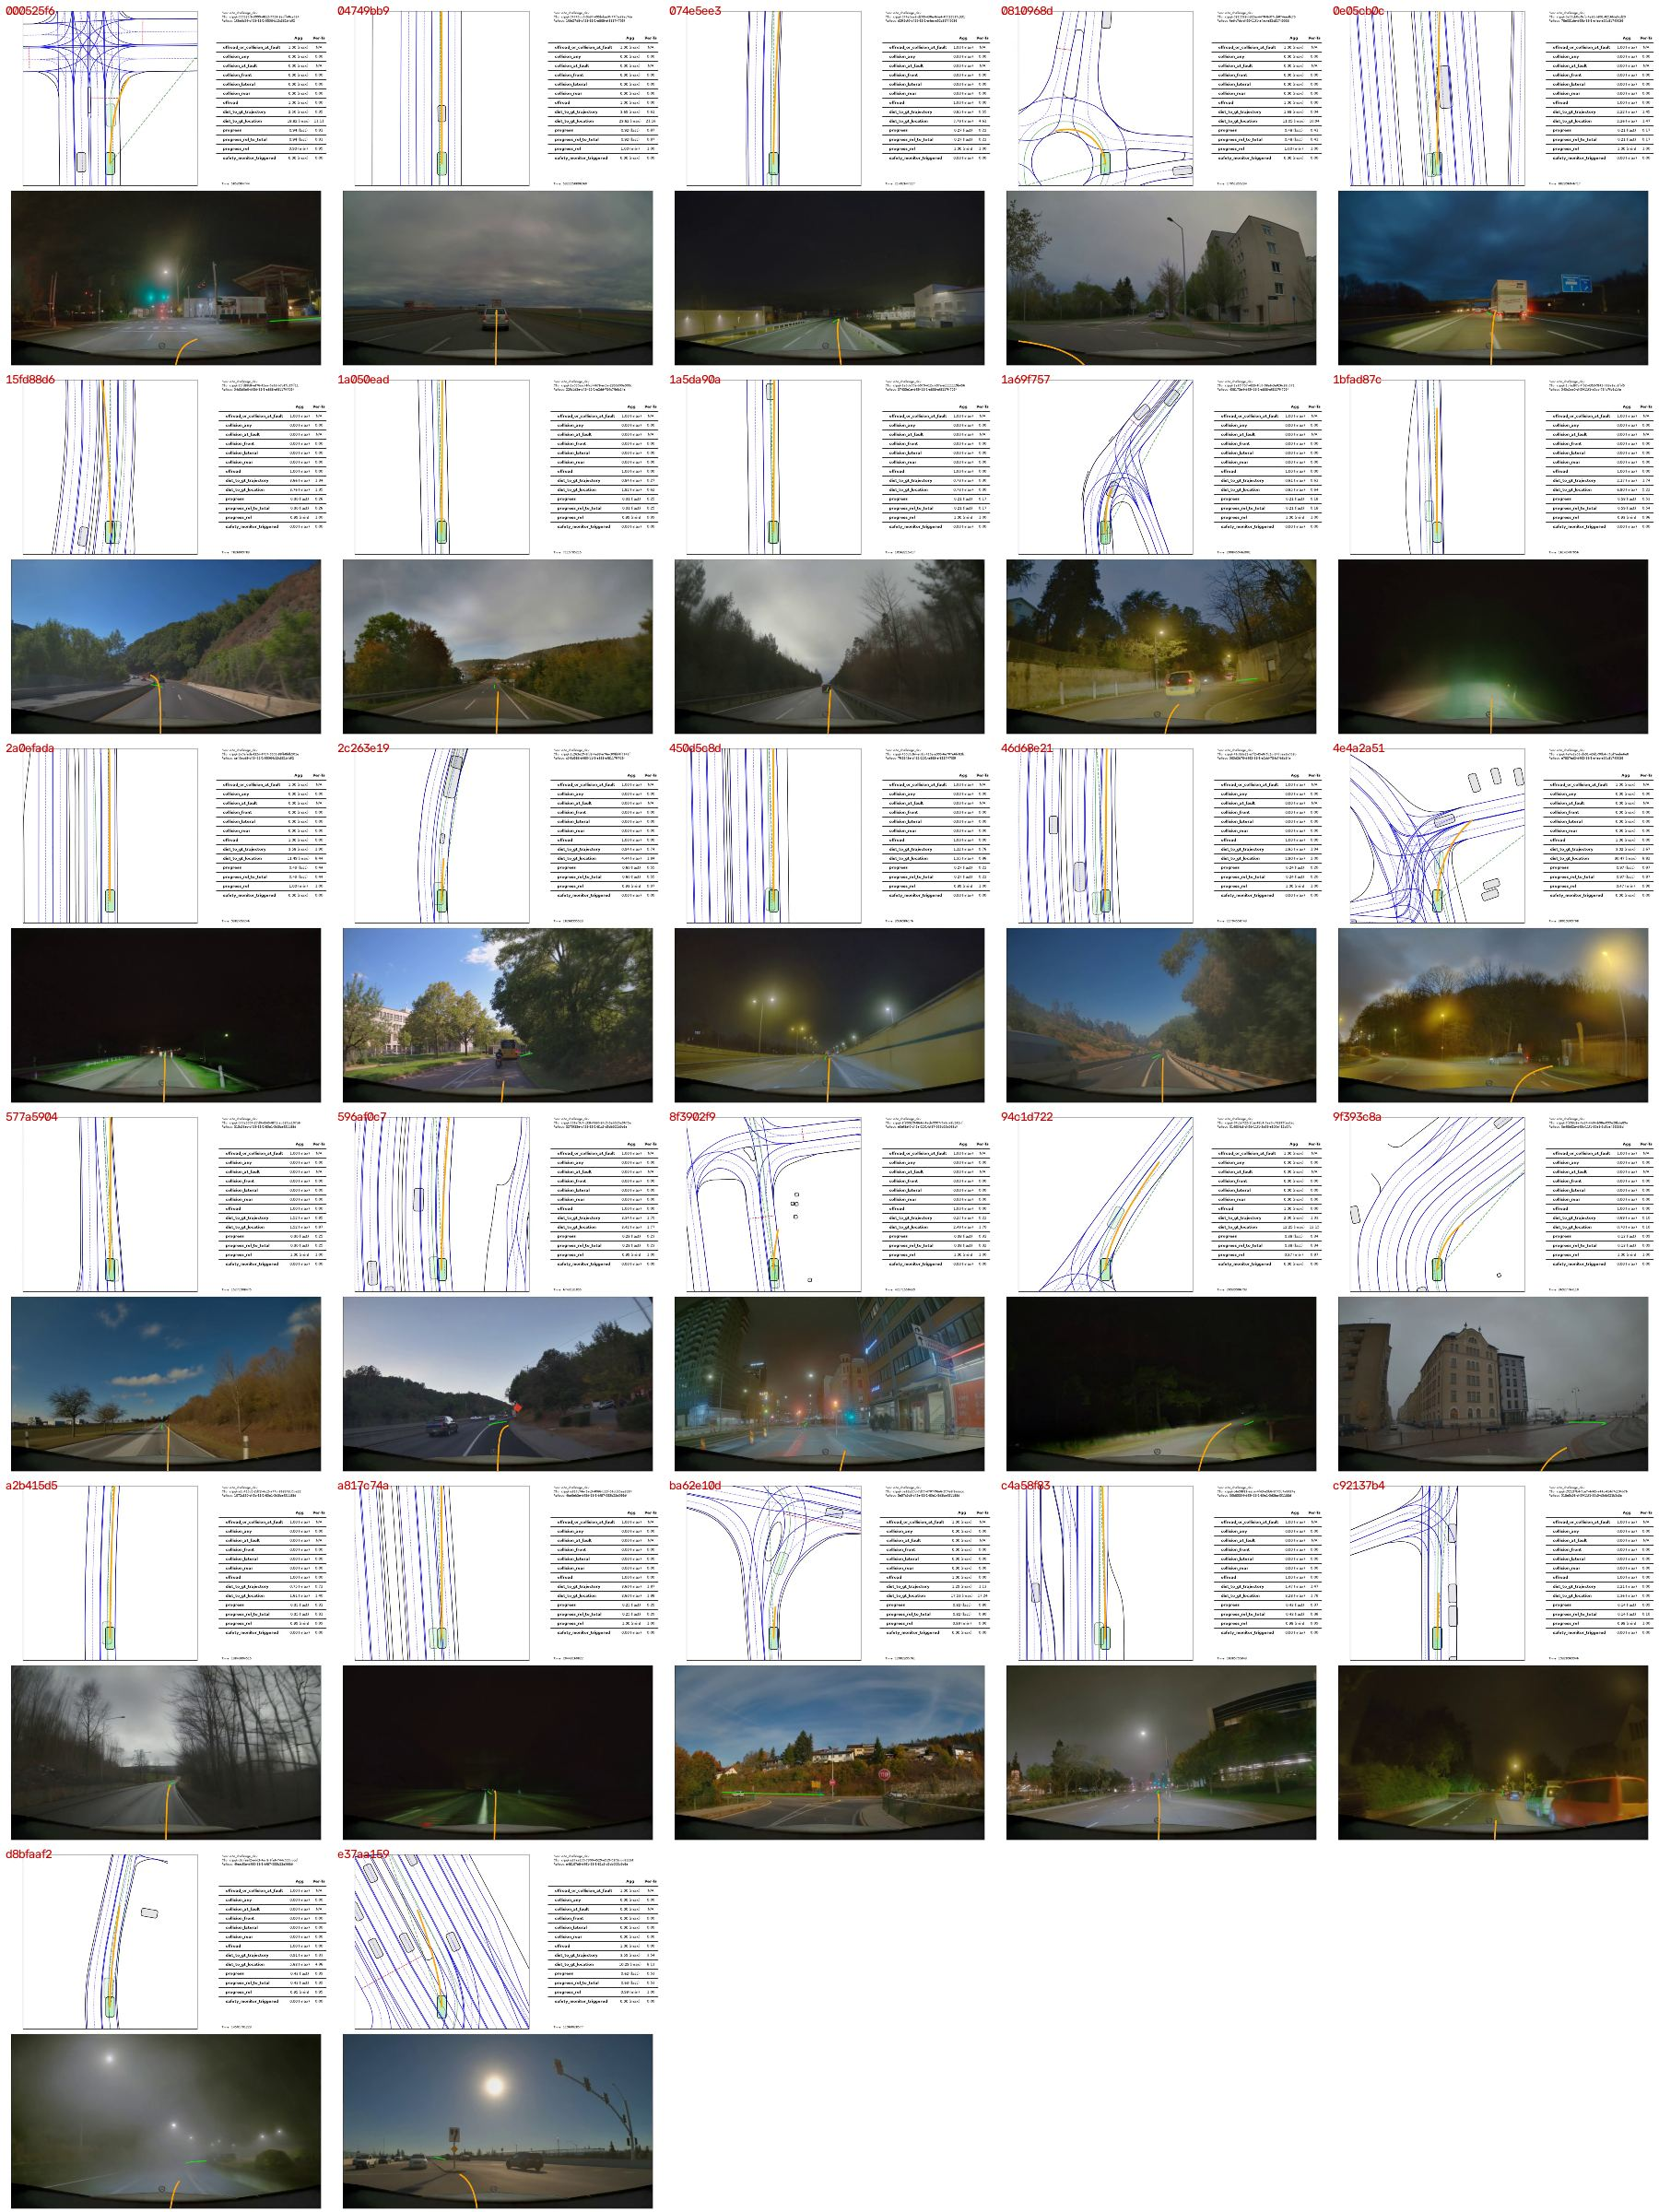
\includegraphics[width=\linewidth]{figures/sheet_offroad.jpg}
\caption{All offroad failures with AEB (first rollout), 0.8\,s before the event.}
\label{fig:sheet_offroad}
\end{figure}

\begin{figure}[h!]
\centering
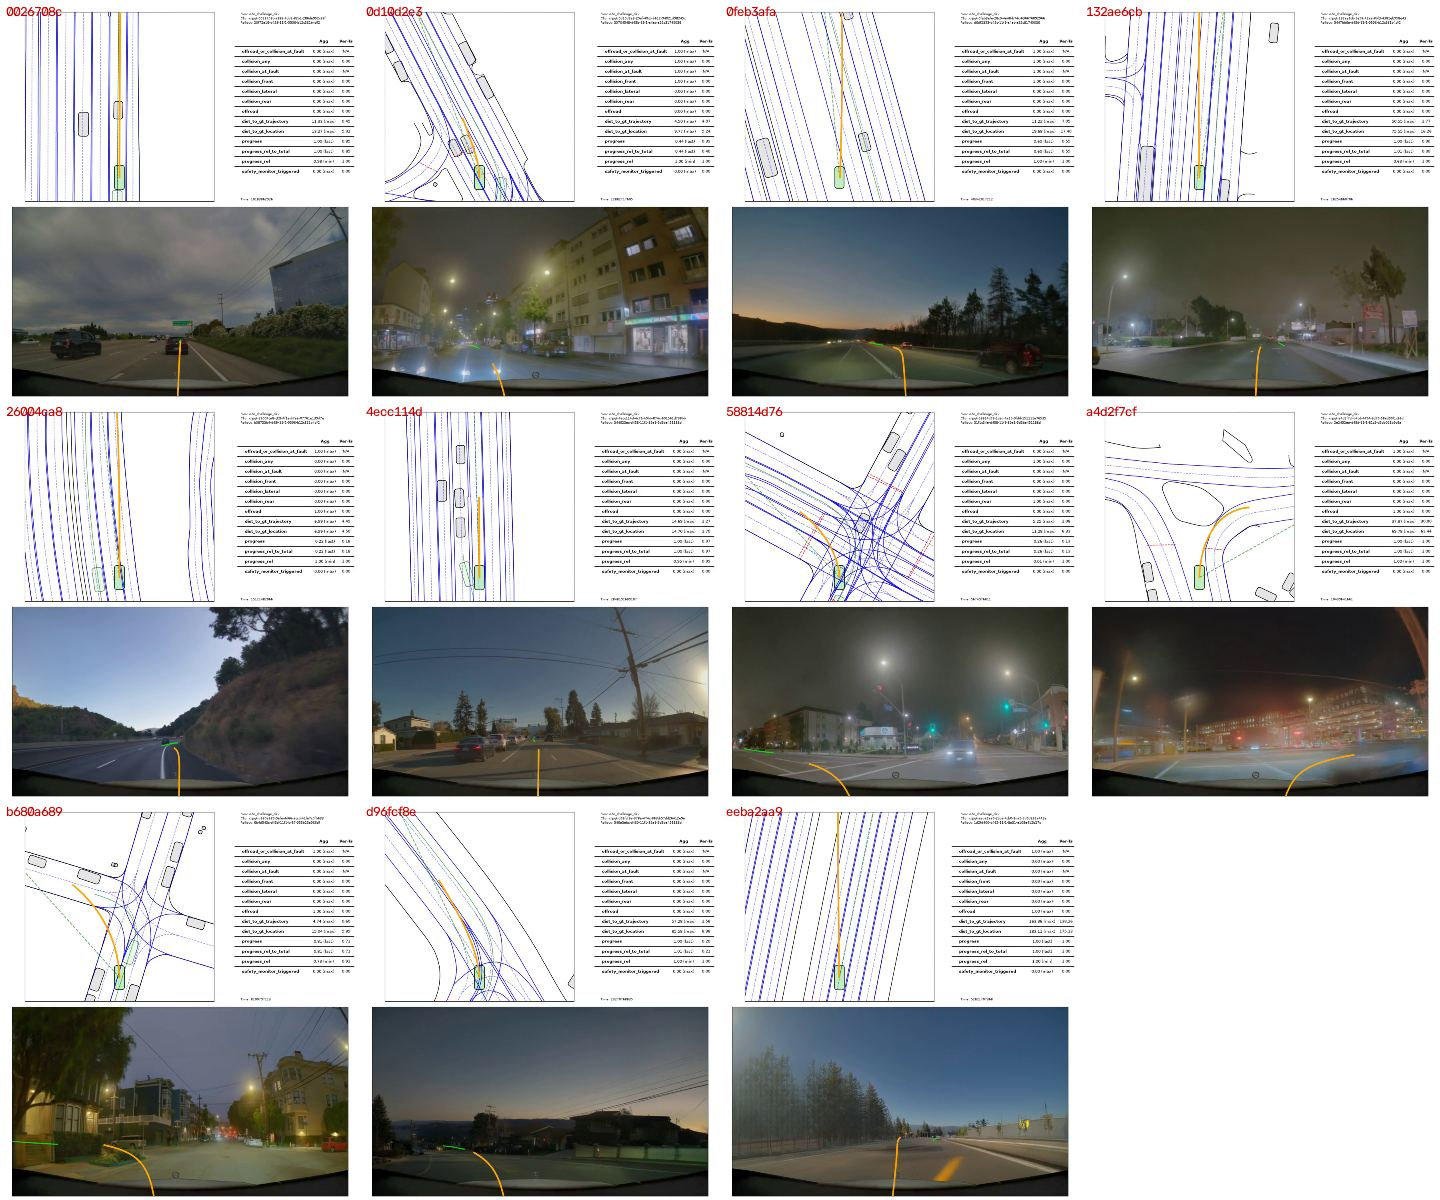
\includegraphics[width=\linewidth]{figures/sheet_exit.jpg}
\caption{All lateral corridor exits with AEB (first rollout), 0.8\,s before the incident or end of scoring.}
\label{fig:sheet_exit}
\end{figure}


\section{Variants evaluated and not submitted}
\label{app:others}
All use the same local protocol and no AEB. These are reported as negative or inconclusive results.
\begin{itemize}\setlength\itemsep{0pt}
\item \textbf{Temporal ensembling (TE4).} In the spirit of ACT~\cite{act}: each new plan is averaged with up to 3 older plans where they overlap in time, each rigidly re-anchored so its pose at the new plan's creation time equals the current pose, with weights $\exp(-0.5\cdot\mathrm{age})$.
\item \textbf{8 samples.} 8 flow-matching samples per plan averaged in the normalized action space.
\item \textbf{hist\_ft.} 3-epoch mask fine-tune from the baseline's final checkpoint: ego-history dropout $p=0.5$ with a presence flag (past $x, y$, heading, speed and all $a_\mathrm{lon}$ zeroed; the current speed is always kept), past-motion dropout after ChauffeurNet~\cite{chauffeurnet}, a dropped target where it is a clip's fallback endpoint, and 300 gate-only steps.
\item \textbf{sig02.} As hist\_ft with a sigmoid mask (initial keep 0.2) and a budget penalty of weight 0.1.
\end{itemize}
Both fine-tunes trained for only 3 epochs.

\begin{table}[h!]
\centering\scriptsize
\caption{Variants we evaluated and did not submit (no AEB), paired as in Table~\ref{tab:app_pairs}, one rollout each against the mean of two.}
\label{tab:app_others}
\begin{tabular}{lccccccc}
\toprule
Comparison & $n$ & Ref. & Run & Diff. & 95\% CI & W/L & $p$ \\
\midrule
Baseline + TE4 vs.\ baseline (2) & 150 & 0.479 & 0.504 & +0.026 & [-0.027, +0.079] & 33/22 & 0.18 \\
Mask + TE4 vs.\ mask (2) & 150 & 0.517 & 0.495 & -0.021 & [-0.082, +0.041] & 25/29 & 0.68 \\
Mask + 8 samples vs.\ mask (2) & 150 & 0.517 & 0.512 & -0.005 & [-0.051, +0.040] & 24/21 & 0.77 \\
hist\_ft vs.\ mask (2) & 150 & 0.517 & 0.495 & -0.021 & [-0.082, +0.037] & 29/26 & 0.79 \\
sig02, 1st vs.\ mask (2) & 150 & 0.517 & 0.505 & -0.012 & [-0.077, +0.055] & 27/28 & 1.00 \\
sig02, 2nd vs.\ mask (2) & 150 & 0.517 & 0.497 & -0.020 & [-0.084, +0.043] & 29/29 & 1.00 \\
\bottomrule
\end{tabular}
\end{table}


\section{Runtime measurements}
\label{app:runtime}
All local measurements share hosts with other jobs and differ from the official evaluator, which runs 16 replicas on 4 GPUs with 2 rollouts per replica. Official numbers appear in submission status. Table~\ref{tab:app_loss} gives the driver telemetry of evaluation runs (recording on, up to 12 rollouts per driver).

\begin{table}[h!]
\centering\scriptsize
\caption{Baked submission images, started without arguments in the sandbox: 2 replicas with 1 session each on one GPU shared with another job, about 27\,s. Times in s.}
\label{tab:app_sub}
\begin{tabular}{lccccc}
\toprule
 & Mean Drive & Planning call & Other calls, mean & Other calls, p50 & Calls with detector \\
\midrule
AEB 10\,Hz & 0.111 & 0.249 & 0.077 & 0.026 & 143/143 \\
AEB 5\,Hz & 0.104 & 0.230 & 0.072 & 0.015 & 82/143 \\
\bottomrule
\end{tabular}
\end{table}

\begin{table}[h!]
\centering\scriptsize
\caption{Saturation test: recorded rollouts replayed into 3 replicas (submission sandbox, no recording) on one RTX 6000 Ada also used by another job, 2 sessions each, with no simulator between calls. This overstates contention; compare rows only. Times in s.}
\label{tab:app_load}
\begin{tabular}{lcccccccc}
\toprule
 & Sessions & Ticks & Mean & p50 & p90 & p99 & Per tick & Wall \\
\midrule
No AEB & 6 & 1071 & 0.294 & 0.001 & 1.457 & 1.512 & 0.322 & 64 \\
AEB 10\,Hz & 6 & 1071 & 0.317 & 0.169 & 0.890 & 1.125 & 0.346 & 71 \\
AEB 5\,Hz & 6 & 1071 & 0.306 & 0.113 & 1.167 & 1.365 & 0.333 & 67 \\
\bottomrule
\end{tabular}
\end{table}


In the saturation test, the mean Drive increases by 8\% at 10\,Hz and 4\% at 5\,Hz relative to no AEB. The absolute values are not model latency: 6 sessions compete for one GPU with no idle time between calls, in contrast with a simulator that spends time rendering.

\section{Sources of the reported data}
\label{app:sources}
Open-loop metrics, training signals and Figs.~\ref{fig:evo_left}--\ref{fig:base_straight} come from W\&B runs \texttt{ccb412c9} and \texttt{03bdfc50} in project \texttt{starVLA\_drive}, both started from commit \texttt{b5c4446} with seed 42. Closed-loop data come from each run's \texttt{aggregate/results-summary.json}, per-step \texttt{metrics.parquet} and \texttt{rollout.asl}. Deployed model code differs from the training commit only by options that are off for this checkpoint (history dropout and fallback-target handling).
